\documentclass[oneside,11pt]{starlink}
\providecommand{\ORACDR}{\textsc{orac-dr}}


% ------------------------------------------------------------------------
% starlink set up
%\title{SUN/258}
\stardoccategory  {Starlink User Note}
\stardocinitials  {SUN}
\stardoccopyright{Copyright \copyright\ 2012 University of British Columbia \& the Science \& Technology Facilities Council}
\stardocnumber    {258.4}
\stardocsource    {sun\thestardocnumber}
\stardocauthors   {Edward Chapin, Andrew G. Gibb, Tim Jenness, David S. Berry, Douglas Scott \& Remo Tilanus}
\stardocdate      {25th February 2015}
\stardoctitle     {SMURF -- the Sub-Millimetre User Reduction Facility}
\stardocversion   {Version 2.0.0}
\stardocmanual    {User's Guide}
\stardocabstract  {
  The Sub-Millimetre User Reduction Facility (\SMURF) is a software
  package for initial reduction of data produced by the ACSIS correlator
  and the SCUBA-2 bolometer array on the James Clerk Maxwell Telescope
  (JCMT). This document describes the \SMURF\ tasks used to process raw
  ACSIS data into data cubes, and raw SCUBA-2 data into images. These
  low-level tasks are used within automated \ORACDR\ pipelines (documented
  elsewhere) that produce calibrated data products. This document is
  intended for users who wish to run the low-level tasks themselves, to
  explore possibilities not provided by the automated pipelines.
}
\starfunders{University of British Columbia \& the Science \& Technology Facilities Council}
\startitlepic{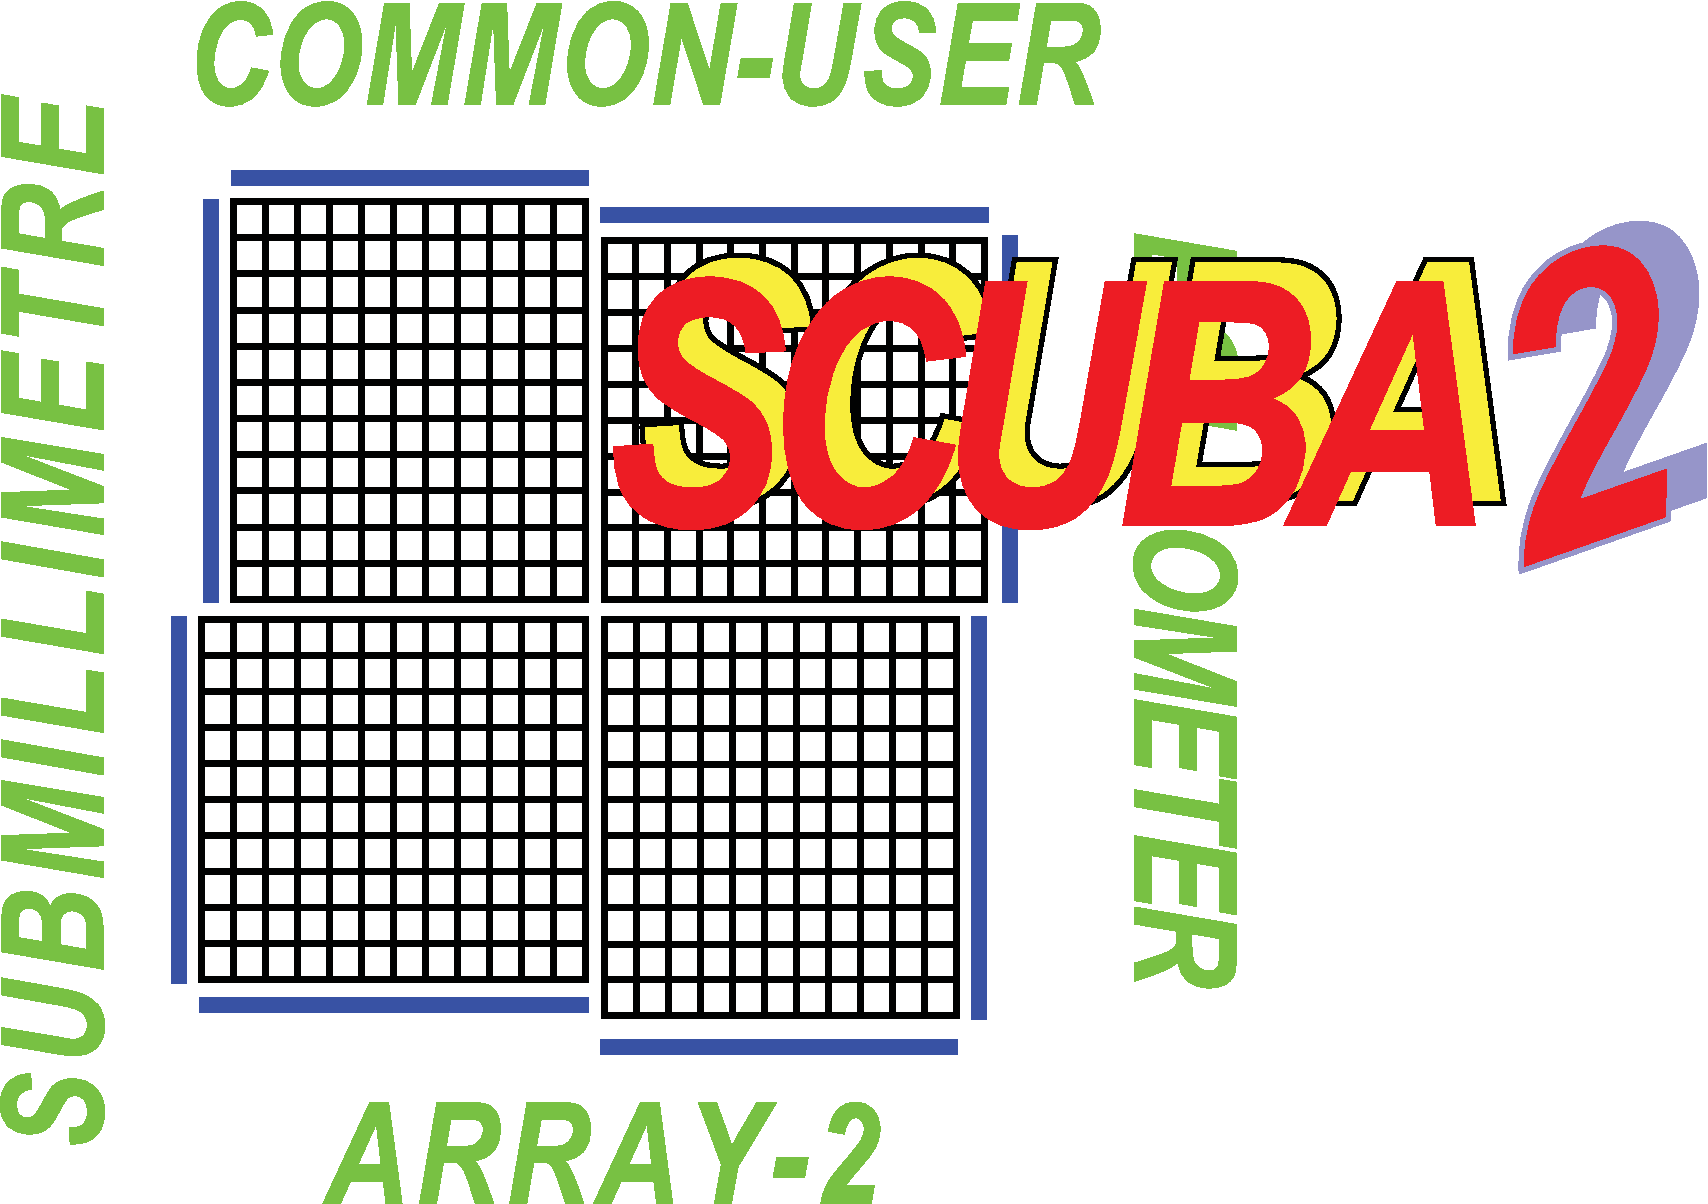
\includegraphics[width=0.55\textwidth]{sun258_logo}}

\begin{document}

\scfrontmatter

\section{\xlabel{introduction}Introduction\label{se:smurfintro}}

This document is aimed at users who wish to perform their own customised
reductions of ACSIS or SCUBA-2 data. It is is expected that most users
will normally prefer to use the higher level facilities provided by
the appropriate \ORACDR\ pipeline.

The main purpose of this document is to provided complete reference
information for all facilities provided by \SMURF. Thus, for instance, it
contains details of \emph{all} available command parameters and configuration
parameters. It is not really intended to be read from start to finish as
a complete document, but rather to be dipped into, as and when needed,
for information about specific parameters or facilities. Most users
will normally refer to this document during the course of reading the
following higher-level documents:

\begin{itemize}
\item \xref{SC/21}{sc21}{}: SCUBA-2 data reduction cookbook (covers the use of
both \SMURF\ and \ORACDR).
\item \xref{SUN/264}{sun264}{}: More details on using the \ORACDR\
SCUBA-2 pipeline.
\item \xref{SC/19}{sc19}{}: SCUBA-2 SRO data reduction cookbook (focuses
specifically on reduction of very early SCUBA-2 data but also contains
some methods and information not yet available in SC/21).
\item \xref{SC/20}{sc20}{pipeline}: Reducing ACSIS data using the \ORACDR\
ACSIS pipeline.
\end{itemize}

After an introductory section covering the mechanics common to using
all \SMURF\ commands, the rest of this document is divided into two main
parts; one dedicated to processing ACSIS data (\cite{acsis}, see Section
\ref{se:acsisdr}) and the other for processing SCUBA-2 data (\cite{scuba2},
see Section \ref{se:sc2dr}).

\subsection{Document conventions}

In an attempt to make this document clearer to read, different fonts
are used for specific structures:
\begin{itemize}

\item Observing modes are denoted by all upper case body text (e.g.\
FLATFIELD).

\item Starlink package names are shown in small capitals (e.g.\ \SMURF);
individual task names are shown in sans-serif (e.g.\ \makemap).

\item Content listings are shown in fixed-width type (sometimes called
`typewriter'). Extensions and components within NDF (\ndfref) data
files are shown in upper case fixed-width type (e.g.\
\ndfcomp{HISTORY}).

\item Text relating to file names, key presses or entries typed at the
command line are also denoted by fixed-width type (e.g.\ \texttt{\%
  smurf}), as are command-line parameters for tasks (which are displayed in
upper case - e.g.\ \aparam{METHOD}).

\item References to Starlink documents, i.e., Starlink User Notes (SUN),
Starlink General documents (SG) and Starlink Cookbooks (SC), are given
in the text using the document type and the corresponding number
(e.g.\ SUN/95). Non-Starlink documents are cited in the text and
listed in the bibliography.

\end{itemize}


\subsection{Using \SMURF}

\SMURF\ is a suite of \starlink\ ADAM tasks (\xref{SUN/101}{sun101}{}
and \xref{SG/4}{sg4}{}) and therefore requires the \starlink\
environment to be defined. For C shells (csh, tcsh), do:

\begin{terminalv}
% setenv STARLINK_DIR <path to the starlink installation>
% source $STARLINK_DIR/etc/login
% source $STARLINK_DIR/etc/cshrc
\end{terminalv}

before using any Starlink commands. For Bourne shells (sh, bash, zsh), do:

\begin{terminalv}
% export STARLINK_DIR=<path to the starlink installation>
% source $STARLINK_DIR/etc/profile
\end{terminalv}

\subsubsection{Starting \SMURF}

Having set up Starlink as described in the previous paragraph, the
\SMURF\ commands are made available by typing \verb+smurf+ at the shell
prompt. The welcome message will appear as shown below:
\begin{terminalv}

% smurf

        SMURF commands are now available -- (Version 1.6.1)

        Type smurfhelp for help on SMURF commands.
        Type 'showme sun258' to browse the hypertext documentation.
        Type 'showme sc21' to view the SCUBA-2 map-making cookbook

\end{terminalv}
This defines aliases for each \SMURF\ command, gives a reminder of the
help command and shows the version number. You can now use \SMURF\
routines or ask for help.

\subsubsection{Getting help}

Access the \SMURF\ online help system as follows:
\begin{enumerate}
\item At the prompt, type \smurfhelp. The welcome message is
  displayed along with a list of available topics.
\item To get information, type the name of an available topic at the
  help prompt.  The next level of help lists information and further
  subtopics.
\item To go to the next level, type the name of a subtopic.
\item Type a question mark, \verb+?+, to re-display the available
  topics at the current level.
\item To go back one level, press \verb+<Enter>+.
\item To exit the help system, press \verb+<Enter>+ until you return
  to the shell prompt.
\end{enumerate}
Further help on the help system maybe obtained by accessing the topic
\verb+smurfhelp+ from within \smurfhelp. If you already know the topic
for which you want help, you can access it directly by specifying it on
the \smurfhelp\ command line, as in the following example:

\begin{terminalv}
% smurfhelp makemap parameters
\end{terminalv}

If an application prompts you for input and you do not know what the
parameter means, you can use \verb+?+ at the prompt for more
information.

\begin{terminalv}
% calcflat
IN - Input flatfield files > ?

CALCFLAT

  Parameters

    IN

      IN = NDF (Read)
         Input files to be processed. Must all be from the same
         observation and the same sub-array.

IN - Input flatfield files >
\end{terminalv}

\subsubsection{\SMURF\ parameters}

\SMURF\ uses named parameters to specify input and output files and
other variables necessary for data processing. There are two types of
named parameter which should not be confused as they are accessed and
specified in very different ways:

\begin{description}
\item[``ADAM'', or ``command line''  parameters:] These can be specified on
the command line when running a \SMURF\ command, in just the same way as when
running other Starlink commands. If no value is supplied on the command
line for a parameter, a default value will be used. If no default value
is available, or if use of a default is not appropriate, then the user is
prompted for a value. The reference documentation for each \SMURF\ command
includes details of each ADAM parameter, and indicates if a default will
be used or not. \KAPPA\ \xref{(SUN/95)}{sun95}{se_param}\ has a
convenient overview of the Starlink parameter system. ADAM parameters are
usually used to specify the main inputs and output for each command, and
to select the main options to be used.

Maybe the most difficult aspect of giving ADAM parameter values on the
command line is handling shell meta-characters. If the parameter
value includes any characters that would normally be interpreted and
replaced by the Unix shell before invoking the requested command, such as
wild-cards, dollars, commas, \emph{etc}, then they must be protected in
some way so that the Starlink software receives them unchanged. This can
be done either by escaping each meta-character (i.e. preceding each one
with a back-slash character - ``\textbackslash'') or by quoting the whole
string. If all else fails, it may be necessary to enclose the parameter
value in two layers of quotes, an inner layer of single quotes and an
outer layer of double quotes. \emph{Note, the above comments only apply for ADAM
parameter values that are supplied on the command line - when supplying a
value in response to a prompt, ths Unix shell is not involved and so shell
meta-characters should not be escaped or enclosed in quotes.}

\item[Configuration parameters:] These are used to fine tune the details
of specific algorithms, and are usually much more numerous than ADAM
parameters. If required, a \SMURF\ command will access an entire group of
configuration parameter settings using a single ADAM parameter usually called
``\aparam{CONFIG}''. The configuration parameter settings can be specified
directly as a comma separated list in response to a prompt for
\aparam{CONFIG}, or may be stored in a text file, the name of which is then
supplied (preceded by a caret - `\verb+^+') when prompted for
\aparam{CONFIG}. Each \SMURF\ command that requires a group of configuration
parameters will document what is needed, and how it can be supplied, in the
reference documentation for \aparam{CONFIG}. Appendix \ref{par:full} describes
individual configuration parameters in detail. \KAPPA\ \xref{(SUN/95)}{sun95}{se_groups}\
has a complete description of the various ways in which groups can be specified.
\end{description}

\subsubsection{\xlabel{sec_msg}Message filter}

All \SMURF\ commands support the `message filter' ADAM parameter
(\aparam{MSG\_FILTER}), which controls the number of messages \SMURF\
writes to the screen when executing routines. The default setting for
the message filter is \verb+normal+. Table \ref{tab:msgfilter} lists
the available values for \aparam{MSG\_FILTER}. Be aware that specifying
\verb+verbose+ or \verb+debug+ will slow down execution due to the
(potentially vast) number of messages written to the terminal. It is
also possible to control message output by setting the
\verb+MSG\_FILTER+ environment variable to one of the values listed in
this table. To hide all messages, a quick option is to add \aparam{QUIET}
to the command line.

\begin{table}
\centering
\begin{tabular}{|c|l|}
\hline
Option  & Description \\
\hline
none    & No messages \\
quiet   & Limited messages \\
normal  & Very few messages \\
verbose & Full messages \\
debug   & Some debugging messages (useful for programmers) \\
all     & All messages regardless of debug level \\
\hline
\end{tabular}
\label{tab:msgfilter}
\end{table}

\subsubsection{\xlabel{files}Working with data files\label{se:files}}

\SMURF\ does not itself enforce a naming scheme on files. However, raw
data from ACSIS and SCUBA-2 obey a well-defined naming scheme. The
convention is as follows: the name is composed of an instrument
prefix, the UT date in the form YYYYMMDD, a zero-padded five-digit
observation number, followed by a two-digit sub-system number (ACSIS
only) and a zero-padded four-digit sub-scan number, all separated by
underscore characters. The file has an extension of \verb+.sdf+. The
instrument prefix for ACSIS is simply ``\verb+a+''. For SCUBA-2 it is a
three-character string dependent on the particular sub-array from which
the data were recorded. The SCUBA-2 sub-arrays are labelled a--d at
each wavelength, which are coded by a single digit (either 4 or 8 for
450 and 850\,$\mu$m data respectively); thus the SCUBA-2 prefix is
\verb+s[4|8][a-d]+.

Example ACSIS file name: a20090620\_00023\_01\_0002.sdf\\
Example SCUBA-2 file name: s8a20090620\_00075\_0001.sdf

Files can be processed either singly or in batches. It is more
efficient to process multiple files at the same time. There are three
ways to specify multiple files:

\begin{enumerate}
\item store the file names in a text file and then supply the
file name, preceded by a caret `\verb+^+', as the value for ADAM
parameter \aparam{IN}.
\item include one or more wild-cards in the ADAM parameter value. Such wild-cards
are expanded by Starlink itself, rather than the Unix shell, and so need to
be protected from shell expansion using quotes or back-slashes as described
earlier.
\item list the file names explicitly, separated by commas (which need to
be quoted).
\end{enumerate}

For more information on specifying groups of objects for input and output,
see the section \xref{\textit{Specifying Groups of Objects}}{sun95}{se_groups}
in the \KAPPA\ documentation (SUN/95). Examples of valid inputs (including the
back-slashes and quotes required to protect the shell meta-characters) are:

\begin{terminalv}
IN=s8a20090620_00075_0001.sdf
IN=s8a20090620_00075_\*
IN=s8a20090620_00075_00\?\?
IN="'file1,file2'"
IN=^myfile.lis
OUT=\*_out
\end{terminalv}

Note that if you are providing a text file containing \emph{output} file names,
those should be listed in the same order as the input file names, otherwise the
processed data will be written under the wrong file names.

\subsection{Data file structure}

Data files for both ACSIS and SCUBA-2 \cite{sc2ic01} use the Starlink N-dimensional
Data Format (NDF, see \ndfref), a hierarchical format which allows
additional data and metadata to be stored within a single file. The KAPPA
\KAPPA\ \xref{(SUN/95)}{sun95}{ap_classified}\ contains many commands for
examining and manipulating NDF structures. A single
NDF structure describes a single data array with associated meta-data.
NDFs are usually stored within files of type ``\verb+.sdf+''. In most
cases (but not all), a single \verb+.sdf+ file will contain just one
top-level NDF structure, and the NDF can be referred to simply by
giving the name of the file (with or without the ``\verb+.sdf+'' prefix).
In many cases, a top-level NDF containing JCMT data will contain other
``extension'' NDFs buried inside them at a lower level. For instance, raw
files contain a number of NDF components which store
observation-specific data necessary for subsequent processing. The
contents of these (and other NDF) files may be listed with
\HDSTRACEref. Each file holding raw JCMT data on disk is also known as a
`sub-scan'.

The main components of any NDF structure are:
\begin{itemize}
\item An array of numerical data (may have up to 7 dimensions - usually 3
for JCMT data);
\item An array of variance values corresponding to the numerical data
values;
\item World Coordinate System information;
\item History;
\item Raw data units (``K'' for ACSIS, ``adu'' (possibly as compressed integers)
for raw SCUBA-2 data,  ``pW'' for flat-fielded SCUBA-2 data, \emph{etc}).
\end{itemize}
For ACSIS, the raw data are stored as $N_{\textrm{chan}} \times N_{\textrm{receptors}} \times N_{\textrm{samp}}$, while SCUBA-2 data are stored as
$N_{\textrm{columns}} \times N_{\textrm{rows}} \times N_{\textrm{samp}}$, where
$N_{\textrm{samp}}$ is the number of time samples in a file.

The files also contain additional NDF components common to both
instruments:
\begin{itemize}
\item JCMT State structure (the telescope pointing record) and other
  metadata that potentially varies for every sample;
\item JCMT Observatory Control System (OCS) configuration, with the
  contents of the XML file used to set up the observation;
\item A ``FITS extension'' containing information in the form of a set of
  FITS (Flexible Image Transport System) header cards, that does not
  change during a sub-scan.
\end{itemize}

The \jcmtstate\ command can be used to extract the time varying
metadata and store it in a tab-separated table
(\xref{TST}{sun190}{ACCESS}) format catalogue.\footnote{This is a
  standard format historically supported by \cursa\ and ESO SkyCat} so
that it can be visualised using \topcat. An example \topcat\ plot of the
telescope motion for a particular observation can be seen in
\ref{fig:topcat}. The JCMTSTATE extension contains information from
the telescope, secondary mirror and real-time sequencer (RTS). ACSIS
observations include environmental weather information and SCUBA-2
observations include SCUBA-2 data (such as the mixing chamber
temperature) and the water vapour monitor (WVM) raw data. \jcmtstate\
converts the telescope and SMU information to additional columns
showing the tracking and AZEL offsets and also converts raw WVM data
to a tau (CSO units). Finally, SCUBA-2 data has additional low-level
MCE information that can be included in the output catalogue using the
`\verb+--with-mce+` option.

\begin{figure}
\begin{center}
\includegraphics[width=1\textwidth]{sun258_scan_pattern}
\caption{The telescope positions during observation number 7 on
  20090107. The plot is created by \topcat\ from the output from
\jcmtstate\ plotting the DRA columns against the DDEC column. The pong
scan pattern is clearly visible.}
\label{fig:topcat}
\end{center}
\end{figure}

The original XML used to specify the details of the observation can be
obtained from any data file using the \dumpocscfg\ command.

The FITS extension is used to store information that either does not
change or changes by a small amount during the course of an observation.
Note that in the particular case of SCUBA-2 data some values in the FITS
extension will change for each sub-scan (i.e. file) of a single
observation. The values in the FITS extension may be viewed with the
\KAPPA\ \fitslist\ command.

Each instrument has further specific components. SCUBA-2 files contain
dark SQUID data, the current flatfield solution, an image of the
bolometers used for heater tracking and possibly information
indicating how to uncompress the raw data. ACSIS files contain
information about the receptors used including their coordinates in
the focal plane.

Output files created by \SMURF\ may contain some or all of these, plus
new components with information about the output data. These are noted
in the description of specific applications. All output files contain
a \ndfcomp{PROVENANCE} extension which provides a detailed record of
the data processing history. Use the \KAPPA\ command \provshow\ to list
the contents.

\subsection{Supported coordinate systems}

\SMURF\ uses AST (\astref) for its astrometry and thus any coordinate
system supported by AST may be used when creating images/cubes. The
default behaviour is to use the system in which the observations
were made (known as the \aparam{TRACKING} system within \SMURF).

\subsubsection{Moving sources}

The mapping tasks \makemap\ and \makecube\ automatically
deal with moving sources. There is no need to deal with moving sources
explicitly for any processing with \SMURF. Maps and cubes made from
moving sources will use a coordinate system that represents \emph{offsets}
from the source centre, rather than absolute celestial coordinates.

\subsection{File sizes and disk space}

Be aware that the raw data files from both instruments may be large
(tens to hundreds of megabytes). Subsequent processing of raw SCUBA-2
time-series data produces output files which are even larger for two
reasons:

\begin{enumerate}
\item The archived raw integer data values are compressed using ``delta''
compression (see \KAPPA\ task \ndfcompress) and must therefore first be
uncompressed before being processed\footnote{This uncompression is
performed automatically when the data is read by any Starlink command - there
is no need to uncompress the data as a separate step.}. The compression ratio
varies from file to file but is usually in the range 2 to 3.
\item The uncompressed data values are then converted from four byte
integer to eight byte floating point.
\end{enumerate}

Thus file size increases in the range 4 to 6 are to be expected. \SMURF\
mapping tasks have the ability to restrict the size of output data files
for manipulation on 32-bit operating systems. For further details, see
the description of the \aparam{TILEDIMS} parameter in the sections on
\makemap\ and \makecube. Processing SCUBA-2 data is faster on 64-bit systems
due to its use of double precision for all calculations.

\section{\xlabel{acsis}ACSIS Data Reduction\label{se:acsisdr}}

SMURF contains a small number of commands specifically directed towards
the reduction of ACSIS data. This section contains an introduction to
each of these commands. The reduction of ACSIS data is described
more fully in \emph{The Heterodyne Data Reduction Cookbook}
(\xref{SC/20}{sc20}{}).

\subsection{The makecube command}

The central step in the reduction of ACSIS data is the conversion of one
or more time-series cubes with \texttt{[spectral channel number, receptor
index, time-slice index]} axes, into a spatial cube with \texttt{[RA, Dec, spectral channel number]} axes\footnote{The RA and Dec axes may
be replaced by axes appropriate for other celestial co-ordinate
systems.}. This step is accomplished using the \makecube\ command.

This command first defines the extent (in both pixels and world
co-ordinates) of the output cube, initialises the output cube to hold
zero at every pixel, and then goes through each receptor sample value in
the input data. For each such sample, it first works out its position on
the sky and its spectral position, using the meta-data in the input
files. It then determines the pixel in the output cube that has the same
spatial and spectral position, and then ``pastes'' the sample value into
the output cube at this central pixel position. This pasting involves
dividing the input sample value up between the output pixels in the
neighbourhood of the central output pixel, and then incrementing each of
these output pixel values by its assigned share of the input sample
value. Various schemes can be used to determine the share assigned to each
output pixel - the simplest and fastest is ``nearest neighbour'' in which
the whole input sample value is assigned to the central output pixel.
Whilst being fast, this scheme can produce small geometric shifts in
feature positions. Other available schemes include a bi-linear scheme
that spreads each input value out linearly between the four closest
output pixels, Gaussian weighting with a given radius, Sinc weighting,
\emph{etc}.

There are many other aspects of the operation of \makecube\ that can be
controlled via various program parameters, some the more important of
which are:

\begin{itemize}

\item The output data can be split up amongst multiple output cubes, thus
reducing the size of each individual cube.

\item The world co-ordinate system used by the output cubes can be
specified. This includes both the nature of the WCS axes themselves and
the details of the tangent-plane projection (pixel size, orientation,
\emph{etc}). If required, optimal values for the projection details can be
determined automatically to produce a regular grid (or as close to a
regular grid as is possible given the input data). Alternatively, the WCS
in the output cube be copied from a specified reference NDF.

\item Output variance values can be calculated either on the basis
of the spread of the input data values that contribute to each output pixel,
or on the basis of the system noise temperature values supplied in the
input NDFs.

\item Input data from specified receptors can be excluded.

\item Input data from specified spectral channels can be excluded.

\item A catalogue can be created holding the spatial position of every
used input sample value.

\end{itemize}

\subsection{The timesort command}

The \makecube\ commands turns time-series cubes into spatial cubes. Each
plane in a time-series cube contains a set of spectra - one for each
used receptor - observed simultaneously at a time given by the position
of the plane on the third axis. It should be noted that the times
associated with this third axis are not guaranteed to increase
monotonically, although that will often be the case. For various reasons,
the writing out of some times slices to the time-series cube may be delayed,
resulting in backwards steps in time along the third axis. This in itself
is not a problem for \makecube\, which makes no assumptions about the
order in which time-slices are stored in the time-series cube. However,
other commands may fail - particularly commands that need to locate the
time-slice index associated with a given time. Such commands assume that
time is a monotonic function of time-slice index, and that therefore the
equivalent of a simple binary chop can be used to locate the index
associated with a given time. These commands will fail with a message
indicating that ``no inverse transformation can be found'' if the
time-series cube contains any out-of-order time slices. Operations that
may produce such a failure include attempting to use \KAPPA\ \wcsalign\
to align two time-series cubes, or displaying a 2D slice of a time-series
cube using \KAPPA\ \display. In these cases, the time-series cube can be
``rectified'' using \timesort. This produces a copy of the cube in which
the time slices are in monotonic order.

In addition, \timesort\ can also be used to assemble and re-order the time
slices from multiple input cubes relating to the same observation, and then
write them out again into a set of time-series cubes, each of a specified
size. In this situation, if a single time slice is split across two
input cubes (which can happen - spectra from some detectors being recorded
in one file and those from the other detectors in another file), they
will be merged together into a single plane in one of the output cubes.


\subsection{The unmakecube command}

The process of converting one or more time-series cubes into a spatial
cube will usually produce some degree of smoothing in the output data due
to multiple input samples contributing to each pixel in the output cube.
This smoothing can sometimes be useful in terms of reducing systematic
differences between the input time-series cubes, such as differing
base-lines. In these cases it is informative to be able to quantify the
effect of this smoothing. The \unmakecube\ command provides this facility
- it creates a set of ``artificial'' time-series cubes from a given
spatial cube. In detail, for each sample position in a given set of input
time-series cubes, a given spatial cube is interpolated to create a new
spectrum, which is then stored at the corresponding position in an output
time-series cube. Thus, any smoothing present in the spatial cube is
transferred into the output time-series cube.

A typical scheme for using unmakecube is:

\begin{enumerate}
\item use makecube to convert a set of ``genuine'' time-series cubes into
a spatial cube.
\item use unmakecube to generate a set of ``artificial'' time-series cubes
from the makecube output spatial cube. The original ``genuine''
time-series cubes are used as templates for the new time-series cubes, so
that they will be aligned sample-for-sample.
\item use the facilities of \KAPPA\ or \GAIA\ to visualise or quantify the
differences between the ``genuine'' and ``artificial'' time-series cubes.
\end{enumerate}

\begin{figure}[htb]
  \begin{center}
    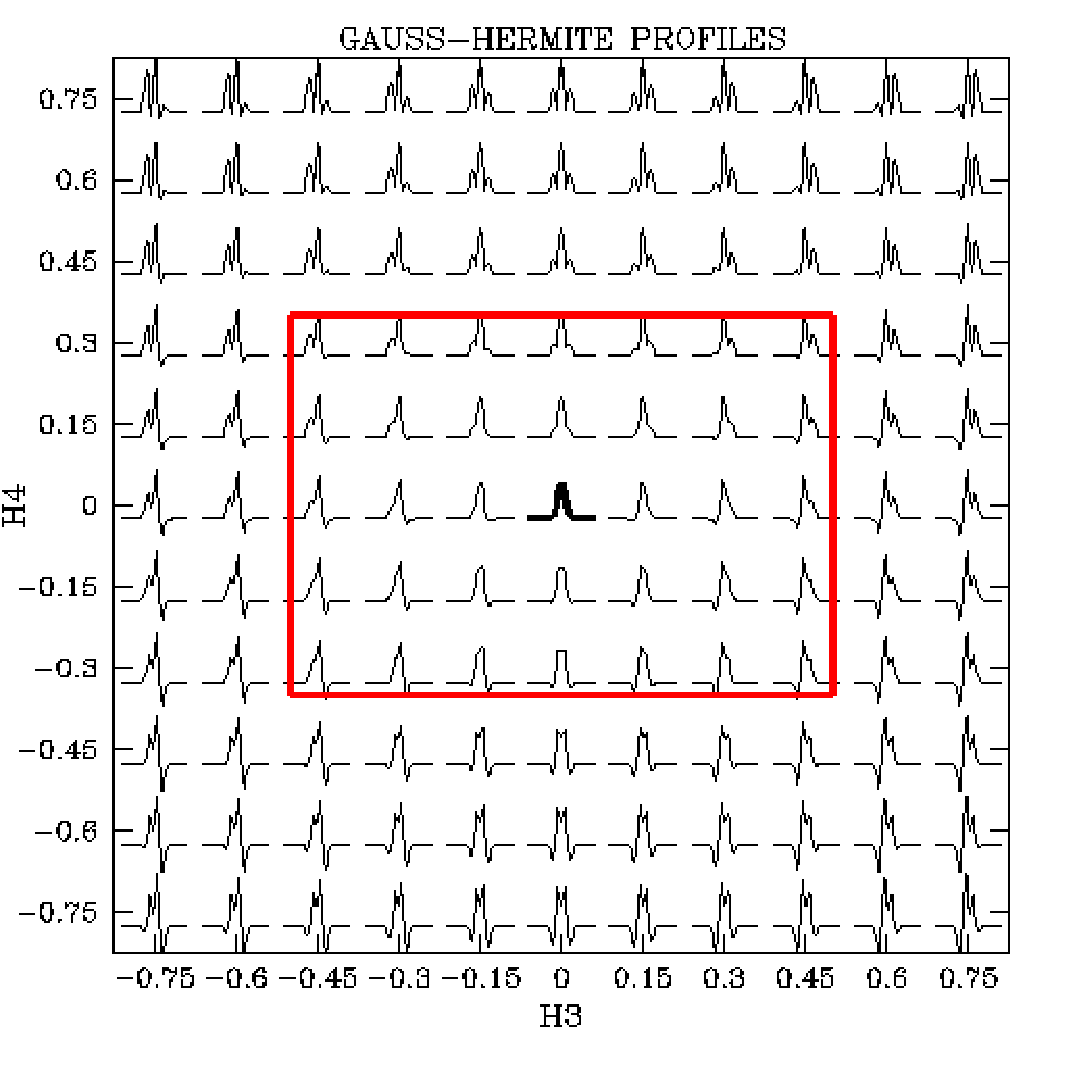
\includegraphics[width=0.8\linewidth]{sun258_gaussherm}
    \caption[Gauss-Hermite shapes]{Fit1d $-$ Gauss-Hermite shapes as a function of the 3rd-order
      ``skewness'' coefficient h3 and the 4th-order the ``peakiness''
      coefficient h4.  the 3rd-order, h3, and the 4th-order, h4,
      coefficients. The red box indicates the limits on acceptable
      values for h3 and h4 as defined in the defaults config file. Note
      that the fitted profile by default is restricted to positive values
      and this will omit the shown negative features (see
      the \cparam{POS\_ONLY} configuration parameter).}
    \label{fig:gaussherm}
  \end{center}
\end{figure}

\subsection{The fit1d command}

The \fitdd\ command fits profiles along a particular axis of a NDF
data file.  It is a generic command that will work on hypercubes with
up to 7 dimensions, but is here discussed in terms of a typical 3-D
ACSIS data-file with axes RA, Dec, and LSR Velocity. Specifically, the fitting
of spectra across the imaged section of the sky. The output of \fitdd\
is a cube with the fitted profiles and ``Component parameter files as
NDF extensions''. Be aware that the input cube is expected to be
baseline subtracted and to have a zero level of 0.

What sets \fitdd\ apart from most other fitting routines is that, by
using ``Component parameter files'' as inputs, it gives individual
control over the fitting at each position. For instance, it is
possible to fit broad lines on the nucleus of a galaxy but narrow
lines everywhere else in the disk. Or to fit multiple components in an
outflow and single components everywhere else in the field. Still,
these types of fits may require a considerable familiarity with
handling, cutting, and pasting NDF files in order to ``create'' the
desired parameter files for input.

\begin{figure}[htb]
  \begin{center}
    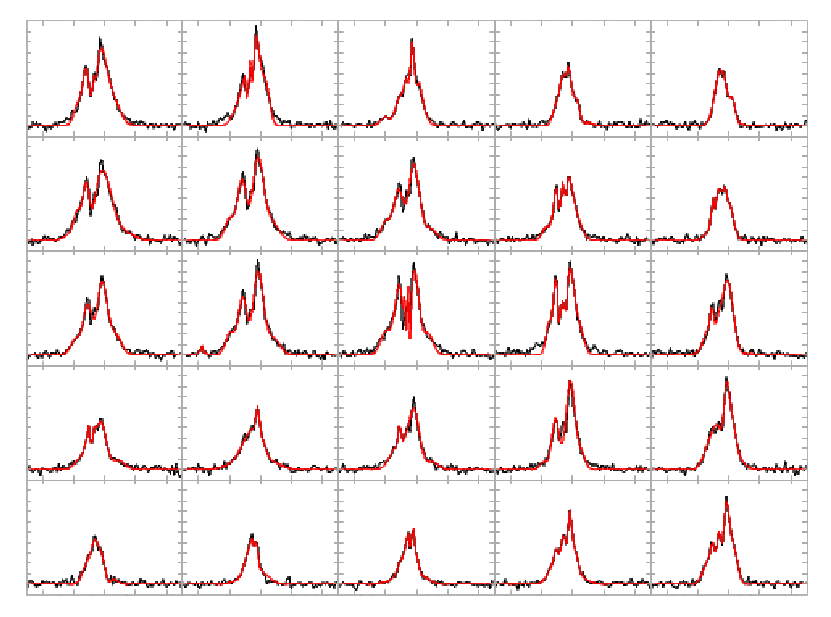
\includegraphics[width=0.8\linewidth]{sun258_fit1d_fits}
    \caption{Fit1d $-$ Black: original profiles; Red: results of a
    3-component Gauss-Hermite2 fit (fitting both h3 and h4, see next section)}
    \label{fig:samplefits}
  \end{center}
\end{figure}

\fitdd\ can also fit more complicated shapes than Gaussians. In
particular, Gauss-Hermite functions are a powerful extension when
fitting profiles that are skewed, peaky, or only approximately
Gaussian. Figure \ref{fig:gaussherm} shows Gauss-Hermite profiles as a
function of the ``skewness'' coefficient h3 and the ``peakiness''
coefficient h4. The red box indicates the limits on acceptable values
for h3 and h4 as defined in the defaults config file. The limits were
chosen such as to exclude fits that look more like multiple components
rather than a distorted single Gaussian, but, admittedly are fairly
arbitrary.

Because of the ability to fit distorted shapes, Gauss-Hermites are
particularly well suited to ``capture'' the maximum amount of emission
from a cube. Figure \ref{fig:samplefits} shows an example of the
quality of the fits that can be obtained. For the shown case \fitdd\
used a 3-component gauss-hermite2 (fitting h3 and h4) function with
the range around the profiles and the remaining configuration
parameters at their default setting.  Collapsing the cube with the
fitted profiles can thus result in an accurate and almost noise-free
white-light or total-emission map. Residuals from the fit can of
course be studied by subtracting the fitted profiles from the original
cube.

\subsubsection{Fitting functions}

\fitdd\ does a one-dimensional fit along each ``profile'' (spectrum),
fitting the number of requested ``components'' concurrently. Function
shapes that can be fitted are ``gaussians'', ``gausshermite1'',
``gausshermite2'', and ``voigt'' functions, which are discussed in
detail in:

\begin{terminalv}
% smurfhelp fit1d fitting_functions
\end{terminalv}

Gauss-Hermite profiles are easiest visualised as the combination of a
Gaussian and decaying asymmetric 3rd-order and/or symmetric 4th-order
polynomials. The 3rd-order polynomial causes a positive bump on one
side and a negative bump on the other side of the main Gaussian,
resulting in asymmetric wings and a skewed shape. By contrast the
4th-order polynomial causes a bump in the centre and steeper slopes
i.e. a peaky shape.

The Gauss-Hermite profiles in \fitdd\ are called gausshermite1,
fitting only h3; and gausshermite2, fitting both h3 and h4 (to fit
only h4, use gausshermite2 and define h3 to be 0 and fixed). The
default in the configuration file for \cparam{FUNCTION} is a
gausshermite2.

To emphasise a number of issues:

\begin{enumerate}
\item Be aware that the art of fitting profiles is not in the fits
  themselves, but rather the initial estimates provided to the
  fit. Supplying user-defined initial estimates for e.g. the width of
  the profiles can greatly influence and help the resulting fit. Also, if
  the initial estimate routine can only find 2 components, the fit will
  also be restricted to fitting that number of components even if the
  user is requesting more.
\item Setting the configuration parameter \cparam{ESTIMATE\_ONLY} to 1
  will skip the fit and produce an output file with profiles based on the
  initial estimates, allowing the user to inspect those. The associated
  Component parameter files could be modified and used as initial estimates
  for a subsequent fit (see next section).
\item Figure \ref{fig:gaussherm} shows that Gauss-Hermites can have
  prominent negative features. By default these are set to zero in the
  fitted spectra: see information in the configuration file for the
  parameter \cparam{POS\_ONLY}.
\item \emph{ONLY for Gaussians} do the fitted parameters correspond
  \emph{exactly} to amplitude, centre, and FWHM! For the other functions
  such correspondence does not exist: while they are related, the
  numerical values are not exact. Users are \textbf{strongly cautioned} to
  keep this in mind. The above-mentioned help for ``fitting\_functions''
  outlines the exact relations.
\item The fitted ``gauss*'' functions can in principle be mixed along a
  profile: i.e. the first component can be fitted as a ``gaussian'', the
  second one as a ``gausshermite2'', etc. Use the \aparam{USERVAL}
  ``User parameter values file'' to accomplish this. It not possible to
  mix in Voigt profiles.
\item However, since \fitdd\ fits concurrently and does not do an
  iterative fit starting with the strongest or centre-most component,
  what is the first, second, etc. component is a fluid concept
  (see next item on sort).  The initial estimates routine orders the
  estimates by decreasing amplitude, but estimates can be quite imprecise.
  The config file options \cparam{SORT} and \cparam{SORT\_ESTIMATE}
  may help in minimising problems (see next point).
\item Sorting of the resulting fits can be done based on the amplitude-like,
  position, or width-like parameter. This can be helpful, but be cautioned
  that it can also complicate things: if there are two components one
  at -10 km/s and one at 10 km/s sorting by amplitude or width can
  result in the parameter file for component 1 to be a mix of the -10
  and 10 features depending on which one was relatively stronger or
  wider. Similarly, sorting by position can result in low-amplitude
  fits of noise spikes to be mixed with stronger components. For more
  precise control try to run the routine iteratively with e.g. a
  different restricted velocity range to try pick out the different
  components. Default sorting is by amplitude.
\item In case multiple components are well separated each can be fitted
separately using \cparam{RANGE}. The resulting Component parameter files
can then be used to generate a combined profile using \fitdd\ with
\cparam{PARCOMP} and \cparam{MODEL\_ONLY}. This is preferred over
simply co-adding the output files with the fitted profiles since it
will put all relevant parameters files in the header of the output
file.
\end{enumerate}

\subsubsection{Component Parameter files}

Besides a cube with the fitted profiles \fitdd\ also outputs so-called
``Component parameter files''. These are added as NDF extensions in
the header of the output file. They can be accessed there directly but
also copied out as independent files:

\begin{terminalv}
% gaiadisp outfile.more.smurf_fit1d.comp_1 outfile.more.smurf_fit1d.comp_2
% ndfcopy outfile.more.smurf_fit1d.comp_0 comp_0
% ndfcopy outfile.more.smurf_fit1d.comp_1 comp_1
etc.
\end{terminalv}

There is a parameter file for each component (``line'') that was
fitted along the profile up to the number of components requested by
the user. These are labelled \ndfcomp{COMP\_1} $\ldots$
\texttt{COMP\_$n$}. \texttt{COMP\_0} is a special diagnostics
component that lists the number of components fitted at each position
and a return code from the fitting routine.

The Component parameter files have 7 images along the axis that was
fitted, with each representing a fitted parameter:

\begin{terminalv}
    COMP_1..N fitted profiles, planes:
               (gaussian)          (gausshermite)        (voigt)
         1 =   amplitude                a                 area
         2 =   position                 b               position
         3 =     fwhm                   c             doppler hwhm
         4 =       -                    h3           lorenztian hwhm `l'
         5 =       -                    h4           amp2area factor `v'
         6 =   (empty)
         7 = function-id (1=gaussian), (2=gausshermite1), (3=gausshermite2)
                         (4=voigt)

    COMP_0 diagnostics info, planes:
         1 = number of components found
         2 = fit error: (see help fit1d)
\end{terminalv}

Thus, for Gaussian fits \ndfcomp{OUTFILE.MORE.SMURF\_FIT1D.COMP\_1(,\phantom{},1)} is
an image of the fitted amplitudes of Component 1 of each profile,
while \ndfcomp{OUTFILE.MORE.SMURF\_FIT1D.COMP\_1(,\phantom{},3)} shows the fitted FWHMs
across the field-of-view.

Much of the (anticipated) use of \fitdd\ derives from the fact that
Component parameter files can be used as input as well: either to
provide initial estimates or fixed values to the fitting routine.
The hierarchy is as follows:
\begin{enumerate}
\item The routine derives initial estimates up to the number of components
requested by the user.
\item These initial estimates are replaced by values from component parameter
files in sequence given (values from the first file specified replace
the initial estimate for the first component, etc.).
\item Any parameter values for component(s) specified by the user in
the ``User parameter values file'' (\aparam{USERVAL}) are then substituted.
\item Finally, a ``fitmask'' is defined based on which parameters are
free to be fitted and which are declared as ``fixed'' in the ``User
parameters values file''. Any non-bad value for a free parameter is treated
as an initial estimate.
\end{enumerate}

The difference between values specified in the component parameter
files and ones declared in the ``User parameter values file'' is that
the former can vary across the field-of-view whereas the latter will
result in the same value being used for all profiles.

In principle a Component parameter file can be created from ``scratch'':
\begin{terminalv}
# Copy a 7-image section from the cube and fill with blanks
% ndfcopy infile'(,,1~7)' temp

# Give the planes pixel coordinates 1..7. Keep the first two dimensions
# at the original value.
% setorigin temp '[-56,-56,1]'

# Fill planes with values: here just use a constant Gaussian (plane 7 = 1)
# with Ampl=10, Pos = 10 km/s, and FWHM = 5 km/s (assuming units of km/s).
% chpix in=temp   out=temp2  section='",,,"' newval=bad
% chpix in=temp2  out=par1   section='",,1"' newval=10
% chpix in=par1   out=par12  section='",,2"' newval=20
% chpix in=par12  out=par123 section='",,3"' newval=5
% chpix in=par123 out=comp_1 section='",,7"' newval=1

# Generate a cube with the model profiles using fit1d with model_only=1
% fit1d in=infile out=model rms=1 parcomp=comp_1 \
%       config='"^/star/bin/smurf/smurf_fit1d.def,model_only=1"'
\end{terminalv}

Obviously, this is not a very practical example given that the profile
is the same across the field: setting values in the user definition
file for component 1 would achieve the same. However, with dedicated
software or a tediously long script running chpix for every position a
sophisticated model could, in principle, be created. For instance if a
feature shifts in velocity across the field, it could be isolated and
fitted by supplying a parameter file with a shifting initial estimate
for the position of the peak.

\begin{figure}[htb]
  \begin{center}
    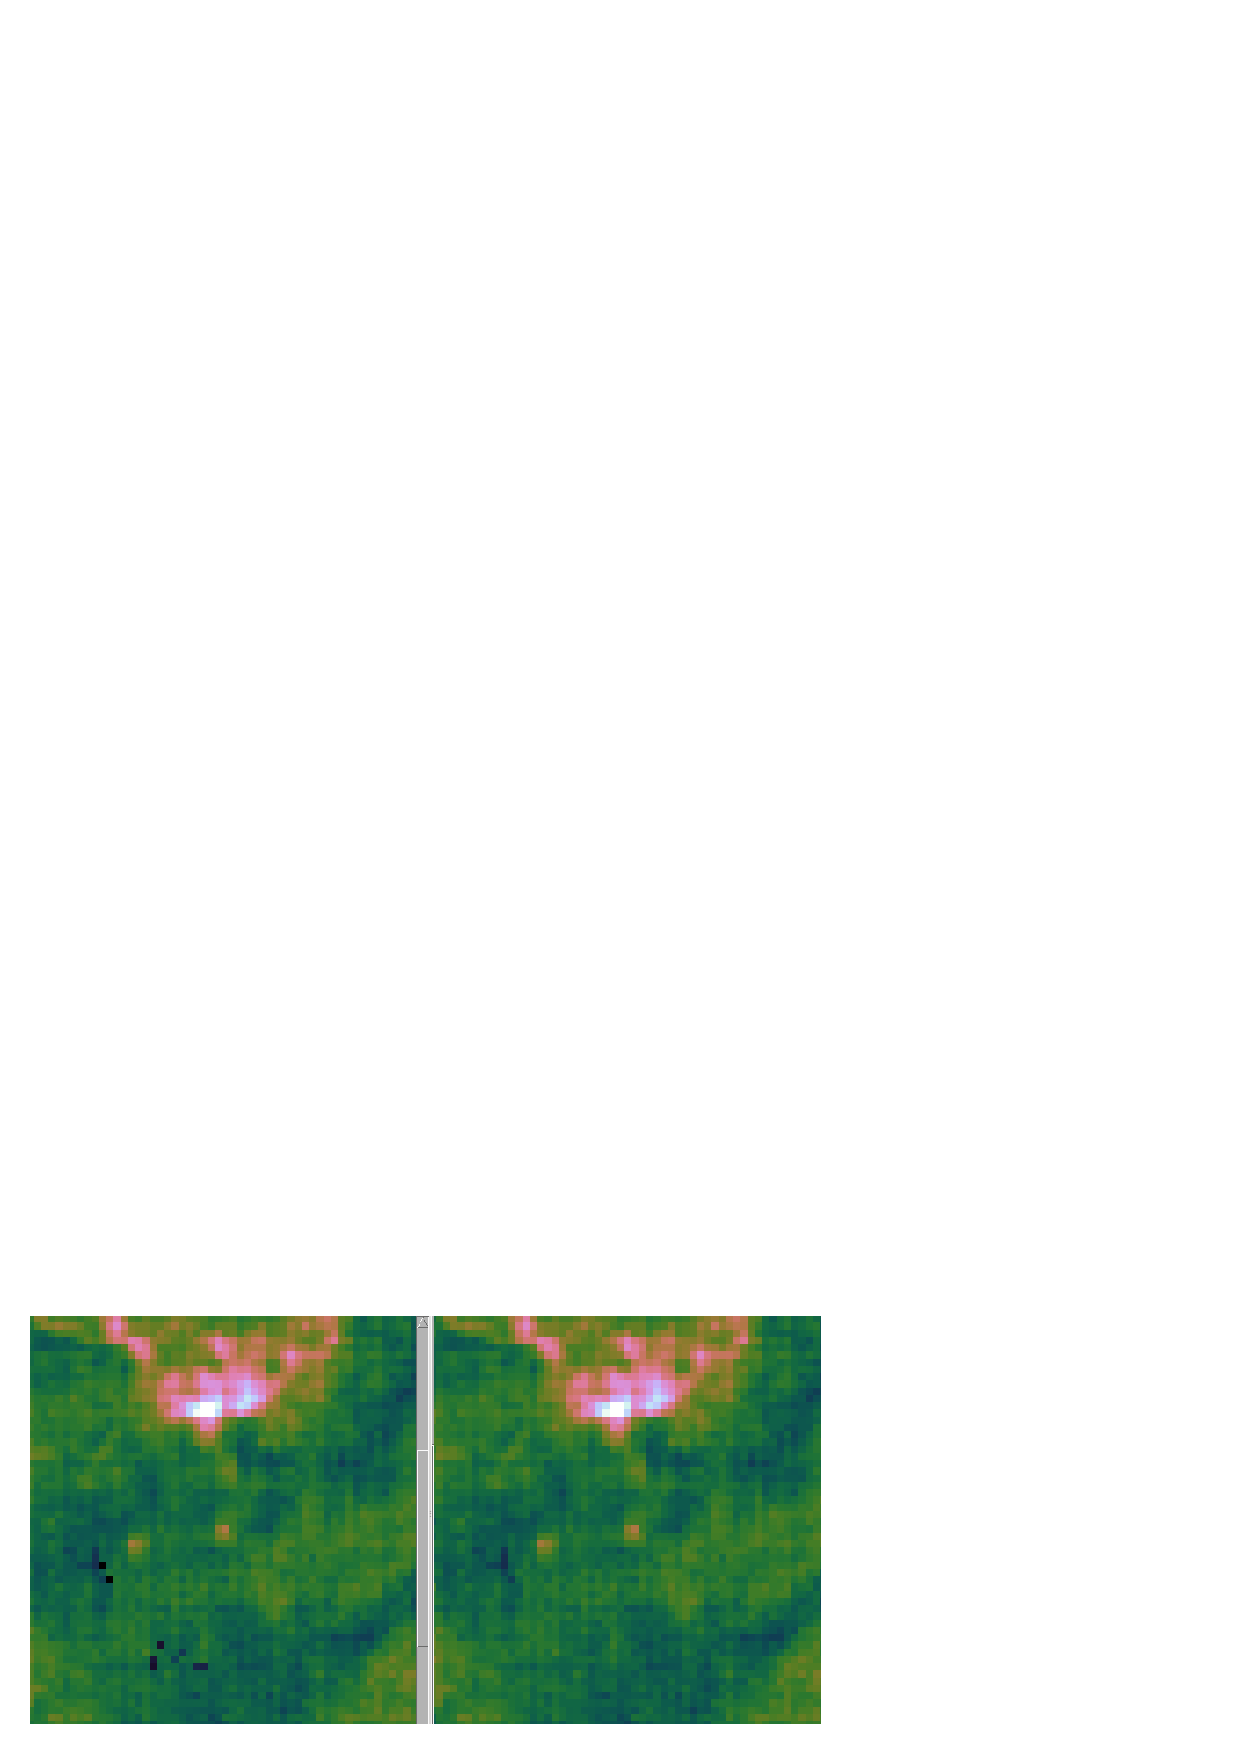
\includegraphics[width=0.8\linewidth]{sun258_fit1d_fixfit}
    \caption{Fit1d $-$  {\it Left:} Section of a parameter file showing
      originally fitted amplitudes; {\it Right:} Amplitudes after using a
      ``fixed'' parameter file from the original fit as initial estimates
      for a subsequent fit.}
    \label{fig:fixfit}
  \end{center}
\end{figure}

Another situation where manipulation of parameter files can be useful
is when parameter files from previous fits require corrections. For
instance, in case it is possible to identify the troublesome locations
by thresholding with \KAPPA\ \thresh, replacing those with bad values; and
\KAPPA\ \fillbad\ can be used to interpolate from surrounding values.

Figure \ref{fig:fixfit} shows an example. On the left is the a section
of the Amplitude plane of a parameter file resulting from a
1-component fit of a Gaussian. In a few positions problems can be seen
(actually due to a secondary component).  These points were isolated
using \thresh\ on the Position plane of the parameters and be
interpolated over using \fillbad. The ``fixed'' parameter file was
then used to provide initial estimates for a subsequent file,
resulting in the fitted Amplitudes on the right.

\begin{terminalv}
% fit1d in=infile out=outfile rms=0.22 config=^fit1d.def
% ndfcopy outfile.more.smurf_fit1d.comp_1 comp_1
% thresh comp_1'(,,2)' out=pos thrlo=2 thrhi=5 newlo=bad newhi=bad
% fillbad pos out=pos_fix
% paste comp_1 p1=pos_fix out=comp_1_fix
% fit1d in=infile out=outfile rms=0.22 config=^fit1d.def parcomp=comp_1b_fix
\end{terminalv}

These fairly simple examples are presented to illustrate the use of
``Component parameter files'', but more elaborate schemes are
possible. For instance, a section of a parameter file that fits broad
lines in the nucleus of a galaxy can be pasted into a parameter file
with narrow fits in the remainder of the disk. We'll leave further
examples to to the imagination of the reader.

\section{\xlabel{scuba2}SCUBA-2 Data Reduction\label{se:sc2dr}}

SCUBA-2 was designed to have two primary observing modes where the
telescope is either stationary relative to the source (DREAM, STARE
and typically when the FTS or polarimeter are in use), or moving (SCAN).
In fact, the DREAM/STARE modes have never been commissioned, and so only the
SCAN mode is functional at the time of writing.  For this reason further
information about DREAM/STARE modes has been relegated to appendix
\ref{se:dsworkflow}.

Two general approaches may be taken to producing maps from SCUBA-2 data
using \SMURF\ commands. By far the easiest approach is to use \makemap\
command to do everything. In this method, the entire job of creating a
map, in units of pW, from raw uncalibrated data is handled in a single
command. This includes all of the data pre-processing steps, as well as
generating the final map.

The alternative approach is to use a range of individual calls to
different \SMURF\ task to perform each of the pre-processing steps,
followed by using \makemap\ to create the final map from the
pre-processed data. This method may be useful if the user wishes to
interact and view each step of the reduction, although the final maps are
generally not of `science grade' quality. The individual \SMURF\ tasks
used in this approach to perform the pre-processing are described in
Section \ref{se:arraycal}. Note, these tasks are not necessary in the usual
case where \makemap\ is used to perform equivalent pre-processing.

Regardless of how the pre-processing is done, the \makemap\ command will
be required to create the final map.  Two methods are available when
running \makemap\ (selected using ADAM parameter \aparam{METHOD}):

\begin{itemize}
\item REBIN: A simple re-binning algorithm that just pastes the cleaned and
flat-fielded bolometer values into the output map.
\item ITERATE: An dynamic iterative method that divides each cleaned and
flat-fielded data value into a number of distinct components, one being an
estimate of the astronomical signal, and the others being various
systematic noise components. The map is then created by pasting just the
component representing the astronomical signal into the output map.
\end{itemize}

The systematic noise in SCUBA-2 data is usually so great that the REBIN
method is inadequate for all but very bright compact sources (bright
enough to be detected in one sample and smaller than the field of view of
the array). In practice, the ITERATE method will give superior results,
though it is more computationally intensive. For this reason, the REBIN
method should never be used other than in exceptional circumstances, and
further discussion of REBIN is relegated to appendix \ref{se:rebin}.

In all normal circumstances, use the dynamic iterative map maker method
described in Section \ref{se:dimm}.

\subsection{Choosing input data files}
In addition to on-sky data files, each observation usually includes
other \emph{calibration data files} such as flatfield ramps and noise
fields\footnote{The type of data in any individual file is recorded in
the \texttt{SEQ\_TYPE} FITS header.}. It is usually safe to include all
the files from an observation, whether on-sky or calibration, when
running a \SMURF\ command, as \SMURF\ will sort them all out and only use
the appropriate type of file for the operation being performed.

\subsection{\xlabel{arraycal}Array calibration and characterisation\label{se:arraycal}}

This section describes the individual \SMURF\ commands that can be used
to perform the pre-processing steps required prior to making a map from
SCUBA\_2 data.  It is usually simpler to supply the raw data direct to
\makemap\ without first using these commands, in which case
\makemap\ will automatically perform the required pre-processing.

Data from array calibration observations (such as FLATFIELD and NOISE)
are processed with \SMURF. NOISE observations are used to identify
bolometers which are not in spec, from which a bad-bolometer mask can
be created. There is usually no need to re-process flatfield data
since the results have already been applied to subsequent observations, but
the techniques are included here for completeness. Both NOISE and
FLATFIELD observations can be done with the shutter closed or with the
shutter open.\footnote{Skydip observations are not available at the
  time of writing}

\subsubsection{\xlabel{flatcal}FLATFIELD\label{se:flatcal}}

FLATFIELD observations are processed with the \calcflat\ command. The
input data must be from the same observation and the same
sub-array. The data are a series of frames in which the current
supplied to the internal pixel heaters is varied about a nominal value
(see the FITS keyword \texttt{PIXHEAT}). \calcflat\ solves for the
optimum heater setting given a list of resistances for each bolometer
and a reference resistor value. The list of resistances is mandatory
and requires knowledge of the sub-array performance. However, a file
with suitable default values is included with the installation of
\SMURF: \texttt{\$STARLINK\_DIR/share/smurf/resist.cfg}.

The output from processing a FLATFIELD observation is a data file
(named automatically if not supplied) which contains the flatfield
solution in the NDF extension \texttt{.MORE.SCUBA2.FLATCAL}, the same
location as for the raw data. The main data array for this output file
is a three-dimensional array containing the reference-subtracted
measurements for each heater setting ($N_{\textrm{row}}\times N_{\textrm{column}} \times N_{\textrm{heat}}$).

In addition to generating the flatfield solution, \calcflat\ can also
create a responsivity image for the current sub-array. The
\aparam{RESP} parameter may be specified to store the
responsivity. The responsivity has units of amperes per watt
(A/W). Since each observation contains the flatfield, it is possible
to extract the responsivity data from any file by using the \calcresp\
command.

If for some reason this flatfield should be applied to existing data
files the \copyflat\ command can be used to copy from the file
generated by \calcflat. This is sometimes useful if a flatfield was
accepted by mistake and it needs to be corrected.

\subsubsection{NOISE}

NOISE observations are designed to check that the bolometers are
operating within specifications. This is achieved by calculating the
power spectrum and looking at the mean power between two frequencies
(usually 2 and 10 Hz). Excessively noisy bolometers are noted and a bad
bolometer mask generated.  The \calcnoise\ command can be used to
analyze any SCUBA-2 time series. It can be used to generate both a
noise image (in pA/rt(Hz)) and a NEP image (in W/rt(Hz)) from raw
data. The noise image will be the image in the main part of the data
file and the NEP image will be in the .MORE.SMURF.NEP extension. If
the data have been flat-fielded the NEP image extension will not be
written since the primary image will already be in power units. A
noise ratio image (.MORE.SMURF.NOISERATIO) is also created to give an
indication of the mean power relative to the power at a particular frequency.

Bad bolometer masks are supported by the \flatfield, \extinction,
\remsky, and \makemap\ tasks through the \aparam{BBM}
parameter. A mask can be generated from the noise images using the
\KAPPA\ \thresh\ command.

\subsubsection{Comparing multiple noise or flatfield observations}

Sometimes you will find that you have many noise or responsivity
images from multiple observations and you would like to investigate the
bolometer stability. The \stackframes\ command can make this simple as
it lets you convert a directory of 2-d images into one data cube where
each frame is sorted by time. Once you have this cube you can load it
into \GAIA\ for easy visualization, use \KAPPA\ \collapse\ with
different estimators, or plot variations using \KAPPA\ \clinplot\ or \mlinplot.

\subsection{\xlabel{dimm}Dynamic Iterative Map-Maker\label{se:dimm}}

The Dynamic Iterative Map-Maker (DIMM) method within the \makemap\
command is the preferred tool for producing maps of SCUBA-2 total power
data obtained in SCAN mode\cite{sc2ana006}. The DIMM is capable of
performing all of the required data pre-processing steps, as well as
solving iteratively for multiple signal components (including the image
of the astronomical sky) using a single call to the \makemap\ task.

As the telescope scans around the sky, each bolometer is sampled around
200 times a second to produce a stream of bolometer values\footnote{This
stream of values is usually down-sampled to a lower frequency so that
individual samples are separated by a distance similar to the pixel size
in the final map.}. The pixel values in the final map are in units of pW
and represent the mean of the time-series bolometer values (after
conversion into pW, down-sampling and removal of systematic noise) that
fall in each pixel.

See Chapin \emph{et. al.} \cite{dimm} for a full description and analysis of the
nature and behaviour of the Dynamic Iterative Map-Maker. Alternatively,
see the SCUBA-2 cookbook (\xref{SC/21}{sc21}{dimm}) for shorter and more
introductory description.

When using \makemap\ with the \aparam{Method=Iterate} option (which is
the default and so does not need to be specified explicitly), it is first
necessary to create a plain text file containing settings for any required
configuration parameters. They can be listed explicitly in the form
`keyword=value', or they can be ``inherited'' from another file by
including the file name preceded by a caret `\verb+^+'. These two methods
can also be combined, with later parameter settings over-riding earlier
parameter settings. Any parameters that are not assigned a value using
one of these two methods will revert to a default value, as listed in
Appendix~\ref{par:full}.

Appendix~\ref{par:full} gives details of \emph{all} the available
configuration parameters - there are quite a lot! Many of these are of
little interest to the majority of \SMURF\ users as they control either
experimental features of the map-maker, or features that should not
normally be changed. The SCUBA-2 cookbook contains a \xref{much reduced
list of configuration parameters}{sc21}{selpars} that are more likely to
be of interest to the majority of users.

Various pre-defined configuration files are included with \SMURF. The
file \texttt{dimmconfig\_jsa\_generic.lis} within directory
\texttt{\$STARLINK\_DIR/share/smurf/} is a useful starting point,
although better results can often be obtained by using a configuration
file tuned to the specific sort of astronomical object being observed
(see the other \texttt{dimmconfig...} files in the same directory). The
SCUBA-2 cookbook (\SMURFcook) describes other ways in which these
``config files'' can be customised.

The basic command to make a map is as follows:
\begin{verbatim}
% smurf
% makemap in=^input.lis out=mapname config=^config.lis
\end{verbatim}

where \texttt{input.lis} is a text file containing the paths to all the
input raw data files for a single observation, one per line, and
\texttt{config.lis} is a text file containing your choice of
configuration parameters. Note, all the input data files should relate to
the same waveband - 450 or 850 - and the same observation.

Many other options are available - see the list of ADAM parameters for
\makemap\ for details. Maybe the most commonly used alternative option is
to use a non-default pixel size. To do this assign the required pixel
size, in arc-seconds, to the ADAM parameter \aparam{PIXESIZE} when
running \makemap:

\begin{verbatim}
% smurf
% makemap in=^input.lis out=mapname config=^config.lis pixsize=3
\end{verbatim}

\subsection{Speeding up map-making by re-using previously cleaned data}

If you want to compare configurations by making several maps from a
single observation, each using a different configuration for the
iterative stages, you can save considerable time by using pre-cleaned
data each time you run \makemap.

\emph{Note, this is only appropriate if the differences between the
various configurations affect only the iterative stage of the map-making
process. If any changes affect the cleaning stage, then it is clearly
inappropriate to re-use the cleaned data from a previous run.}

There are two possible ways to generate the pre-cleaned data:

\begin{enumerate}

\item Use the \SMURF\ \clean\ task. You can run \clean\ in exactly the
same way you would run \makemap\ but instead of creating a map, it
creates a set of files containing cleaned and concatenated time-series
data that can then be supplied as input to \makemap. Any parameters in
the configuration file that do not relate to cleaning are ignored by
\clean\, so you can conveniently use the same file that you would supply
when running \makemap. The ADAM parameter \aparam{OUT}, which specifies
the names of the output data files, can conveniently be set to
``\texttt{*\_cln}'', in which case the output files names will be copies
of the input file names with the addition of ``\texttt{\_cln}'' to the
end. There will usually be fewer output files than input files because
the data from multiple input files will be concatenated together into a
single file. However, data for different wavebands (450 or 850 $\mu$m)
will always be stored in separate files.

\item Alternatively, you can ask \makemap\ to generate the cleaned data.
To do this, you should add \cparam{exportclean=1} to the \makemap\ configuration
file. In addition to the output map, \makemap\ will then also create one or
more files in the current directory with the suffix ``\texttt{...\_cln.sdf}''
containing the cleaned and concatenated time-series data - the earlier part of
these file-names will be derived from the names of the input raw data
files. \emph{Note, remember to remove \cparam{exportclean=1} from your
configuration before running \makemap\ again.}

\end{enumerate}

Then for your subsequent runs of \makemap\, you specify the cleaned data
generated by one of the above two methods as the input, using ADAM
parameter \aparam{IN}. In addition, you must add \cparam{doclean=0} to
the configuration, which prevents \makemap\ from attempting to clean the
already cleaned input data.

\section{Acknowledgments}

The authors are grateful for the documentation written by Maria Kelly
on which the SCUBA-2 part of this SUN was originally based, and
Christa van Laerhoven for an earlier version. The SCUBA-2 simulator
code was originally written as a standalone application by Dennis
Kelly at the UK Astronomy Technology Centre and converted to a \SMURF\
task by Jen Balfour.

% End of main text


\begin{thebibliography}{}

\bibitem{archibald}
Archibald~E.~N., et~al., 2002, MNRAS, 336, 1

\bibitem{acsis}
Buckle~J.~V., et~al., 2009, MNRAS, 399, 1026

\bibitem{dimm}
Chapin~E.~L., et~al., 2013, MNRAS, 430, 2545
\htmladdnormallink{doi:10.1093/mnras/stt052}{http://dx.doi.org:10.1093/mnras/stt052},
\htmladdnormallink{arXiv:1301.3652}{http://arxiv.org/abs/1301.3652}

%\bibitem{sc2cook}
%Thomas~H.~S., Currie~M.~J., 2014, \textit{The SCUBA-2 Data Reduction Cookbook},
%\xref{Starlink Cookbook 21}{sc21}{}

%\bibitem{srocook}
%Chapin~E.~L., et~al., 2010, \textit{The SCUBA-2 SRO Data Reduction Cookbook},
%\xref{Starlink Cookbook 19}{sc19}{}

%\bibitem{kappa}
%Currie~M.~J., 1997, {\it KAPPA -- Kernel Application Package},
%\xref{Starlink User Note 95}{sun95}{}

%\bibitem{gaia}
%Draper~P.~W., 1997, {\it GAIA -- Graphical Astronomy and Image
%Analysis Tool},
%\xref{Starlink User Note 214}{sun214}{}

\bibitem{scuba2}
Holland~W.~S., et~al., 2006, Proc. SPIE, 6275, 45

\bibitem{jenness}
Jenness~T., et~al., 2002, MNRAS, 336, 14

\bibitem{sc2ic01}
Jenness~T., Gibb,~A., 2007, \textit{Data Acquisition/Data Reduction
  Pipeline Interface Control Document}, SCUBA-2 Data Reduction
document SC2/SOF/IC210/01

\bibitem{dream}
Le~Poole~R.~S., van~Someren~Greve~H.~W., 1998, Proc. SPIE, 3357, 638

\bibitem{sc2ana001}
Scott~D., 2003, {\it Map-making in different noise regimes}, SCUBA-2
  Data Reduction document SC2/ANA/S210/001

\bibitem{sc2ana006}
Scott~D., 2005, {\it Scan Mode Data Reduction Strategies for
  SCUBA-2}, SCUBA-2 Data Reduction document SC2/ANA/S210/006

\bibitem{sc2ana005}
Scott~D., Van Engelen~A., 2005, {\it Scan Mode Strategies for
  SCUBA-2}, SCUBA-2 Data Reduction document SC2/ANA/S210/005

\bibitem{sc2ana002}
Van Engelen~A., 2005, {\it Analysis of Atmospheric Emission using
  SHARC-II Data and Implications for the SCUBA-2 Simulator},
  SCUBA-2 Data Reduction document SC2/ANA/S210/002

\bibitem{sc2ana004}
Van Engelen~A., Scott~D., 2005, {\it A Correlation Study using SCUBA
  Data, with implications for SCUBA-2 data reduction},
  SCUBA-2 Data Reduction document SC2/ANA/S210/002

%\bibitem{ast}
%Warren-Smith~R.~F., Berry~D.~S., 2009, {\it AST -- A Library for
%  Handling World Coordinate Systems in Astronomy},
%\xref{Starlink User Note 211}{sun211}{}

%\bibitem{ndf}
%Warren-Smith~R.~F., Berry~D.~S., 2009,
%{\it NDF -- Routines for Accessing the Extensible N-Dimensional Data
%  Format},
%\xref{Starlink User Note 33}{sun33}{}

\end{thebibliography}

\section{Release Notes}

\subsection{2015A}
\begin{itemize}
\item This document has been over-hauled, removing or relegating
information that is no longer relevant, or is repeated in other documents.
\item New commands: JSATILEMOC.
\item An experimental scan synchronous noise (SSN) model has been added
to MAKEMAP.
\item The amount of multi-threading in MAKEMAP is reduced automatically if doing so
allows chunking to be avoided.
\item The number of chunks used to make a SCUBA-2 map is now recorded in the
FITS extension of the map.
\item MAKEMAP can now be told to abort if chunking would be used.
\item The \texttt{dimmconfig.lis} configuration file has been deprecated. It
should no longer be used either directly or as the basis for derived
configuration files. Configurations that previously would have inherited from 
\texttt{dimmconfig.lis} should instead rely on the default parameter values 
listed in \texttt{\$SMURF\_DIR/smurf\_makemap.def}.
\end{itemize}

\subsection{2014A}
\begin{itemize}
\item New commands: JSASPLIT, JSAJOIN, JSADICER, JSATILEINFO,
JSATILELIST, CHECKCOORDS, FTS2MASKMAP and FITSMERGE.
\item New MAKEMAP configuration parameters: AST.SKIP, CHUNKWEIGHT,
COM.FREEZE\_FLAGS, COM.SIG\_LIMIT, FLT.FILT\_ORDER, FLT.RING\_BOX1, HITSLIMIT,
xxx.ZERO\_SNR\_FFCLEAN, xxx.ZERO\_SNR\_HIPASS, xxx.ZERO\_SNR\_LOPASS (``xxx'' =
AST, FLT, COM).
\item New MAKEMAP ADAM parameters: JSATILES, ITERMAPS, INTOPTION.
\item New MAKECUBE ADAM parameters: JSATILES, POSERRFATAL.
\item New configuration files: \texttt{dimmconfig\_fix\_blobs.lis} and
\texttt{dimmconfig\_fix\_convergence.lis}.
\item Several values have been changed in \texttt{dimmconfig\_bright\_extended.lis}.
\end{itemize}

\subsection{Hikianalia}
\begin{itemize}
\item New commands: SKYLOOP and CONFIGMELD.
\item If multiple types of mask are requested for any of the AST, FLT
and COM models (e.g. ZERO\_LOWHITS and ZERO\_MASK both specified),
they will now be combined into a single mask. Previously, only one
of the requested masks would be used.
\item Up to three external masks can now be specified using ADAM parameters
REF, MASK2 and MASK3. The ZERO\_MASK configuration parameter can be set
for the AST, FLT or COM model, to indicate which ADAM parameter to use.
\item The dimmconfig.lis file now uses maptol to specify the convergence
criterion rather than chitol.
\item The \texttt{textttdimmconfig\_bright\_extended.lis} file now inherits from
\texttt{dimmconfig.lis}, rather than \texttt{dimmconfig\_bright.lis}. This means
that the values used for COM.CORR\_TOL, COM.GAIN\_ABSTOL, COM.GAIN\_TOL, DCTHRESH and
NOISECLIPHIGH have changed. In addition, \texttt{dimmconfig\_bright\_extended.lis}
now sets the value of FLT.FILT\_EDGE\_LARGESCALE to 600 arc-seconds for
both 450 and 850 um. Previously, the defaults of 600 (at 450 um) and 300
(at 850 um) provided by \texttt{dimmconfig.lis} were accepted. {\bf Thus, the filter
size has changed from 300 to 600 at 450 um.}
\end{itemize}

\subsection{Kapuahi}
Many changes - the most significant were.
\begin{itemize}
\item New commands: UNMAKEMAP, SC2MAPFFT, SC2FILTERMAP, MCEHEAD2CAT, FIT1D.
\item The QLMAKEMAP command has been removed.
\item A new, more stable, common-mode estimation has been introduced into MAKEMAP.
\item More code has been multi-threaded, making MAKEMAP significantly faster.
\item Pointing corrections for the input raw data can now be specified via a
text file, using new parameter POINTING.
\item CONFIG parameters that specify a number of samples can now also be given
in terms of seconds.
\item New CONFIG parameter "COM.PERARRAY" allows a separate common mode signal
to be estimated and used for each sub-array.
\item The COM model can now be masked to omit source samples from the common
mode estimation.
\item The FLT model can now be masked to omit source samples when estimating
the low frequency background of each bolometer time stream.
\item SNR masks for the AST, COM and FLT models can now be taken down to much
lower levels without introducing isolated noise spikes into the mask
(using "xxx.ZERO\_SNRLO" parameters).
\item A bug has been fixed that caused the memory requirements to grow
monotonically when running MAKEMAP repeatedly as a monolith (e.g. from
ORAC-DR or ICL).
\item Updated Water Vapor Monitor calculation. The WVM samples are now smoothed
before being used.
\item Setting config parameter "DOWNSAMPSCALE" to -1 will auto-scale to the pixel
size. This is now the default.
\item New config parameter "MAPTOL" provides a map-based scheme for
testing convergence.
\item New config parameter "NOI.BOX\_SIZE" allows the estimate of the noise
within a bolometer time stream to vary with time.
\item JCMTSTATE2CAT now calculates telescope speed.
\item CALCNOISE  now accepts a map-maker config file for pre-cleaning.
The default config includes common-mode removal.
\item CALCNOISE now calculates the effective noise and NEP.
\end{itemize}

\subsection{Kaulia}

Supports compressed SCUBA-2 data files taken since February 2011.

\begin{itemize}
\item CALCQU - a new command to create Q and U values from SCUBA-2
  fast-spinning polarimeter time-series data files.
\item MAKECUBE
\begin{itemize}
\item Now allows the spatial reference pixel in the output cube to be
  specified by the user.
\item Setting \texttt{TRIM=YES} now modifies any user-supplied
  \texttt{LBND}/\texttt{UBND} values to remove borders of bad pixels.
\end{itemize}
\item MAKEMAP
\begin{itemize}
\item The loading and flatfielding of raw data on multi-core systems
  is now faster.
\item The focal plane distortion model has been updated to cover the
  entire focal plane.
\item A new parameter (\texttt{TRIM}) has been added to allow borders
  of blank pixels to be removed from the output map.
\item A bug has been fixed so that a request to perform just one
  iteration (\texttt{numiter=1}) is honoured.
\end{itemize}
\end{itemize}

\subsection{Namaka}

Major updates to \SMURF\ to support SCUBA-2 data processing.

\begin{itemize}
\item Polynomial fitting to flatfield data is now the default.
\item Fast flatfield ramps are now supported. These are taken at the
  start of every observation.
\item New scripts: smas analyzes "short maps" to investigate high
  frequency seeing/pointing variations
\end{itemize}

\subsubsection{MAKEMAP (iterative)}

\begin{itemize}
\item Maps from small chunks of the time series can now be written
  out. Specify the ``shortmap'' parameter.
\item Typos in config parameters are now trapped and the defaults can
  be seen in file \texttt{smurf\_makemap.def} in
  \texttt{\$SMURF\_DIR}. The actual parameters that are used (the
  merge of the supplied dimmconfig and the defaults) are now stored in
  the history of the output map.
\item Enhanced common-mode removal algorithm which can now break the
  time series into smaller chunks.
\item Enhanced spike removal using a rolling median calculation
\item Enhanced step correction.
\item Output map now includes QUALITY flags to indicate areas that
  have been set to 0 by the map-maker.
\item The map-maker now reports the details of the flagging every iteration.
\item Config files have been re-written to include the standard config
  with explicit overrides. This makes it easier to see what is being
  changed.
\item Major improvement to the speed of calculating the world
  coordinates of every bolometer.
\item Correctly switch to the CSO tau fits header in the absence of WVM data.
\end{itemize}

\subsubsection{SC2CLEAN}

\begin{itemize}
\item The parameter DCBOX has been renamed DCFITBOX.
\item DCBAD and DCFLAGALL parameters have been removed.
\end{itemize}

\subsubsection{SC2FFT}

\begin{itemize}
\item Add NGOOD parameter.
\item Can now calculate an average power spectrum.
\end{itemize}

\subsubsection{STACKFRAMES}

\begin{itemize}
\item Fix some bugs associated with maps of different sizes and with
  missing metadata.
\item Propagate QUALITY properly.
\end{itemize}

\subsection{Hawaiki}

First official release supporting SCUBA-2 raw data (rather than simulated data).

\subsubsection*{New applications}
\begin{itemize}
\item New command CALCNOISE for calculating the noise properties of a SCUBA-2 observation.
\item New command COPYFLAT to copy a flatfield from one SCUBA-2 observation to another.
\item New command STACKFRAMES for taking a collection of 2-D images
  (eg noise images or responsivities) and placing them into a time
  series cube.
\end{itemize}

\subsubsection*{Modified applications}
\begin{itemize}
\item SC2FFT will now concatenate all related files before calculating the FFT.
\item MAKECUBE can now avoid generating very thin tiles when tiling is enabled.
\item MAKECUBE now uses offset sky co-ordinates in the output cube if,
  and only if, the input tracking system is (Az,El) or geocentric
  apparent (RA,Dec).
\item JCMTSTATE2CAT now calculates DRA and DDEC columns to indicate
  arcsecond offsets from base position. Additionally DAZ and DEL are
  now given as offsets from BASE rather than offsets from the first
  base position. For SCUBA-2 files JCMTSTATE2CAT will now optionally include
  MCE header information and will calculate the tau dynamically from the
  raw WVM data.
\end{itemize}

\subsection{Nanahope}

\subsubsection*{Global changes}
\begin{itemize}
\item Improve description of SCUBA-2 processing routines for Nanahope
  Starlink release.
\item A summary of input observations is now presented.
\item If an output file is derived from multiple observations the
  output FITS header will now include start and end information (such
  as date and airmass from the oldest observation and date and airmass
  from the newest observation).

\end{itemize}

\subsubsection*{New applications}
\begin{itemize}
  \item New command CALCRESP for calculating responsivities from
    flatfield solutions.
\end{itemize}

\subsubsection*{Modified applications}
\begin{itemize}
  \item MAKECUBE can now fix up most issues associated with older ACSIS data from 2006 and 2007.
  \item MAKECUBE output catalogues can now contain additional JCMTSTATE information by using the EXTRACOLS parameter.
  \item TIMESORT is now significantly faster.
  \item MAKECUBE, MAKEMAP and QLMAKEMAP are now multi-threaded by default on multi-processor machines.
  \item MAKECUBE now issues a warning message if WCS information implied by the RECEPPOS and FPLANEX/Y values in an input NDF is inconsistent.
  \item TIMESORT can now handle single time slice data cubes.
  \item Many enhancements to SCUBA-2 functionality including support for bad pixel masks and interpolated darks.
 \item jcmtstate2cat now reports AZ and EL as well as DAZ and DEL.
\end{itemize}

\subsubsection*{Bug Fixes}

\begin{itemize}
\item MAKECUBE formerly mis-interpreted non-zero instrument aperture (INSTAP) values in recent ACSIS data.
\item MAKECUBE now ignores input data values that have negative input Tsys values.
\item TIMESORT now sets the correct pixel origin in the output NDFs.
\end{itemize}

\newpage

\appendix
%\renewcommand{\thesection}{\Alph{section}}%
\ifpdf

\section{\xlabel{ap_summary}An Alphabetical Summary of \SMURF\ Commands
\label{ap:summary}}

\begin{description}[itemsep=0.pt]
\menuitem{ACSIS\_INDEX}{Provide a listing of ACSIS data files in a directory.}
\menuitem{BADBOLOS}{
  Generate a map of random dead bolometers and store in extension of the input file.}
\menuitem{CALCDARK}{
 Calculate the 2d dark frame from a dark observation.}
\menuitem{CALCFLAT}{
 Calculate a flatfield solution.}
\menuitem{CALCNOISE}{
Calculate the noise properties of a SCUBA-2 observation.}
\menuitem{CALCQU}{
Calculate Q and U images from a set of SCUBA-2 time-series data files.}
\menuitem{CALCRESP}{
 Calculate bolometer responsivity from stored flatfield solution.}
\menuitem{COPYFLAT}{
Copy the flatfield solution from one SCUBA-2 observation to another.}
\menuitem{DREAMSOLVE}{
 DREAM solver.}
\menuitem{DREAMWEIGHTS}{
 DREAM weight matrix generation.}
\menuitem{DSUTILS}{
Utility functions for estimating focal plane distortions.}
\menuitem{DUMPOCSCFG}{
Retrieve OCS XML configuration used to generate the raw data.}
\menuitem{EXTINCTION}{
 Extinction correct SCUBA-2 data.}
\menuitem{FIXSTEPS}{
Fix DC steps in a supplied SCUBA-2 time-series NDF.}
\menuitem{FLATFIELD}{
 Flatfield SCUBA-2 data.}
\menuitem{GETTSYS}{
Retrieve TSYS (or TRX) from ACSIS data files.}
\menuitem{GSD2ACSIS}{
 Convert a GSD format DAS data file to an ACSIS format NDF. (beta test)}
\menuitem{GSDSHOW}{
 Display the contents of a GSD file's headers and arrays.}
\menuitem{IMPAZTEC}{
  Import AzTEC NETCDF files and produce SCUBA-2 format data files. (untested)}
\menuitem{JCMTSTATE2CAT}{
Dump JCMTSTATE information to ASCII table.}
\menuitem{MAKECUBE}{
 Regrid ACSIS spectra into a data cube.}
\menuitem{MAKEMAP}{
 Regrid SCUBA-2 data into a map.}
\menuitem{MCEHEAD2CAT}{
 Dump the MCE data header of SCUBA-2 files.}
\menuitem{RAWFIXMETA}{
 Report metadata issues with ACSIS data files.}
\menuitem{RAWPRESS}{
Compress raw data that have not previously been compressed. (test routine)}
\menuitem{RAWRECREATEWCS}{
Attempt to fix corrupt spectral metadata in ACSIS data.}
\menuitem{RAWREWRTSC2WCS}{
Attempt to fix corrupt WCS in raw SCUBA-2 data.}
\menuitem{RAWUNPRESS}{
Uncompress raw SCUBA-2 data.}
\menuitem{REMSKY}{
  Remove Sky signal from SCUBA-2 observations.}
\menuitem{SC2CLEAN}{
 Clean-up SCUBA-2 time series.}
\menuitem{SC2CONCAT}{
 Concatenate files from a single observation into a single file.}
\menuitem{SC2EXPANDMODEL}{
Expand a DIMM model component into a full time-series data cube.}
\menuitem{SC2FFT}{
 Perform a forward or inverse FFT on SCUBA-2 data.}
\menuitem{SC2FILTERMAP}{
Filter a 2-D map.}
\menuitem{SC2MAPFFT}{
Fourier transform 2-D maps.}
\menuitem{SC2PCA}{
Use principal component analysis to identify correlated SCUBA-2 signals.}
\menuitem{SC2SIM}{
SCUBA-2 simulator.}
\menuitem{SCUBA2\_INDEX}{
  Provide a listing of SCUBA-2 data files in a directory.}
\menuitem{SKYNOISE}{
 Generate a simulated sky background.}
\menuitem{SMAS}{
  Analyse shortmaps from the map-maker.}
\menuitem{SMURFCOPY}{
Copy a 2d image out of a time series file.}
\menuitem{SMURFHELP}{
Give help about SMURF.}
\menuitem{STACKFRAMES}{
Stack multiple 2-d images into a 3d cube, optionally sorted by time.}
\menuitem{STARECALC}{
 Calculate a map from a STARE-mode observation.}
\menuitem{TIMESORT}{
 Re-order time slices in a raw data cube into increasing time.}
\menuitem{UNMAKECUBE}{
 Produce simulated time series data from a regridded ACSIS data cube.}
\menuitem{UNMAKEMAP}{
Produce simulated time-series data from a SCUBA-2 map.}

\end{description}
\newpage
\fi

\section{\xlabel{ap_classified}Classified \SMURF\ Commands
\label{ap:classified}}

\SMURF\ applications may be classified in terms of their
functions as follows.

{\large
\begin{center}
\textbf{General Purpose}
\end{center}
}

\begin{description}[itemsep=0.pt]
\classitem{DUMPOCSCFG}
Retrieve OCS XML configuration used to generate the raw data.

\classitem{JCMTSTATE2CAT}
Dump JCMTSTATE information to ASCII table.

\classitem{SMURFHELP}
Give help about SMURF.
\classitem{STACKFRAMES}
Stack multiple 2-d images into a 3d cube, optionally sorted by time.
\end{description}

{\large
\begin{center}
\textbf{SCUBA-2 Data Processing}
\end{center}
}

\begin{description}[itemsep=0.pt]
\classitem{CALCDARK}
 Calculate the 2d dark frame from a dark observation.
\classitem{CALCFLAT}
 Calculate a flatfield solution.
\classitem{CALCNOISE}
Calculate the noise properties of a SCUBA-2 observation.
\classitem{CALCQU}
Calculate Q and U images from a set of SCUBA-2 time-series data files.
\classitem{CALCRESP}
 Calculate bolometer responsivity from stored flatfield solution.
\classitem{COPYFLAT}
Copy the flatfield solution from one SCUBA-2 observation to another.
\classitem{DREAMSOLVE}
 DREAM solver.
\classitem{DREAMWEIGHTS}
 DREAM weight matrix generation.
\classitem{DSUTILS}
Utility functions for estimating focal plane distortions.
\classitem{EXTINCTION}
 Extinction correct SCUBA-2 data.
\classitem{FIXSTEPS}
Fix DC steps in a supplied SCUBA-2 time-series NDF.
\classitem{FLATFIELD}
 Flatfield SCUBA-2 data.
\classitem{MAKEMAP}
 Regrid SCUBA-2 data into a map.
\classitem{MCEHEAD2CAT}
 Dump the MCE data header of SCUBA-2 files.
\classitem{RAWPRESS}
  Compress raw data that have not previously been compressed. (test routine)
\classitem{RAWRECREATEWCS}
  Attempt to fix corrupt spectral metadata in ACSIS data.
\classitem{RAWREWRTSC2WCS}
  Attempt to fix corrupt WCS in raw SCUBA-2 data.
\classitem{RAWUNPRESS}
  Uncompress raw SCUBA-2 data.
\classitem{REMSKY}
  Remove Sky signal from SCUBA-2 observations.
\classitem{SC2CLEAN}
 Clean-up SCUBA-2 time series.
\classitem{SC2CONCAT}
 Concatenate files from a single observation into a single file.
\classitem{SC2EXPANDMODEL}
  Expand a DIMM model component into a full time-series data cube.
\classitem{SC2FFT}
 Perform a forward or inverse FFT on SCUBA-2 data.
\classitem{SC2FILTERMAP}
  Filter a 2-D map.
\classitem{SC2MAPFFT}
  Fourier transform 2-D maps.
\classitem{SC2PCA}
  Use principal component analysis to identify correlated SCUBA-2 signals.
\classitem{SCUBA2\_INDEX}
  Provide a listing of SCUBA-2 data files in a directory.
\classitem{SMAS}
  Analyse shortmaps from the map-maker.
\classitem{SMURFCOPY}
Copy a 2d image out of a time series file.
\classitem{STARECALC}
 Calculate a map from a STARE-mode observation.
\classitem{UNMAKEMAP}
  Produce simulated time-series data from a SCUBA-2 map.
\end{description}

{\large
\begin{center}
\textbf{ACSIS Data Processing}
\end{center}
}

\begin{description}[itemsep=0.pt]
\classitem{ACSIS\_INDEX}
  Provide a listing of ACSIS data files in a directory.
\classitem{GETTSYS}
Retrieve TSYS (or TRX) from ACSIS data files.
\classitem{MAKECUBE}
 Regrid ACSIS spectra into a data cube.
\classitem{RAWFIXMETA}
 Report metadata issues with ACSIS data files.
\classitem{TIMESORT}
 Re-order time slices in a raw data cube into increasing time.
\classitem{UNMAKECUBE}
 Produce simulated time series data from a regridded ACSIS data cube.
\end{description}

{\large
\begin{center}
\textbf{Data Import}
\end{center}
}

\begin{description}[itemsep=0.pt]
\classitem{GSD2ACSIS}
 Convert a GSD format DAS data file to an ACSIS format NDF. (beta test)
\classitem{GSDSHOW}
 Display the contents of a GSD file's headers and arrays.
\classitem{IMPAZTEC}
 Import AzTEC NETCDF files and produce SCUBA-2 format data files. (untested)
\end{description}

{\large
\begin{center}
\textbf{SCUBA-2 Simulations}
\end{center}
}

\begin{description}[itemsep=0.pt]
\classitem{BADBOLOS}
 Generate a map of random dead bolometers and add it as an NDF extension to the input file.
\classitem{SC2SIM}
SCUBA-2 simulator.
\classitem{SKYNOISE}
 Generate a simulated sky background.
\end{description}

\section{\xlabel{ap_full}Full Specifications of all \SMURF\ Commands\label{ap:full}}

These pages describe all the \SMURF\ commands in detail. Default
values for parameters are quoted in square brackets. Empty brackets
indicate a dynamic default will be calculated and inserted at run
time. Parameters for which an array should be supplied (or are
returned) are shown with parentheses after the parameter name. A
number within those parentheses indicates the size of the array.

\sstminitoc{ADAM commands}
\input{../../libsmurf/smurfmon}


\clearpage

\section{Python Scripts}

These scripts use \KAPPA\ and \SMURF\ commands to do the number
crunching, but use Python rather than shell script to glue these commands
together. The parameter system used by these scripts has been designed to
be similar to the ADAM parameter system used by most other Starlink
commands. So for instance, values can be specified by keyword or position
on the command line, and the user will be prompted for any required parameter
values that were not specified on the command line. However, there are some
significant differences, including:

\begin{itemize}
\item The used parameter values are \emph{not} stored in a parameter file for
later use. So for instance, the \KAPPA\ \parget\ command cannot be used
to recover parameter values.
\item Parameters that take logical parameters must always specify their
value using an equal sign (\emph{e.g.} \verb+retain=yes+ rather than
\verb+retain+, and \verb+retain=no+ rather than \verb+noretain+).
\item The documentation for the command may be displayed by running the
command with the \verb+--help+ option on the command line.
\end{itemize}

\sstminitoc{Python Scripts}
\input{../../scripts/scripts}
\clearpage

\section{Other Scripts}

%% These are currently generated manually
\sstminitoc{\ }

\sstroutine{
  ACSIS\_INDEX
}{
  Provide a listing of ACSIS data files in a directory
}{
  \sstdescription{
    Reads ACSIS observation files in a directory and creates an
    index. Standard JCMT directory layout is supported.
  }
  \sstusage{
    acsis\_index   [-v | -h | -d | -o] [-a] [-c] [-e] [-f] [-t/T -r/R -s/S]
         [datadir]
  }
  \sstparameters{
    \sstsubsection{
      $-$all
    }{
      Print information on all files even if the headers are identical. For example,
      include multiple subbands (subsystems) and sub-scans.
    }
    \sstsubsection{
      $-$debug
    }{
      Print debugging information.
    }
    \sstsubsection{
      $-$extended
    }{
      Print extended lines. Can add AZ, EL, pointing offsets and bandwidth.
    }
    \sstsubsection{
      $-$force
    }{
      Force a subdirectory search. If no files are found in the
      directory itself, as would be the case for a raw data tree, the
      program will automatically search subdirecties. This option
      forces the subdirectory search.
    }
     \sstsubsection{
       $-$help
      }{
        Print help information.
      }
      \sstsubsection{
        $-$version
       }{
         Print version information.
       }
       \sstsubsection{
         $-$man
       }{
         Print the full documentation to STDOUT.
       }
       \sstsubsection{
         $-$ocscfg
       }{
         Print the OCS configuration XML file.
       }
       \sstsubsection{
         $-$cal
       }{
         Only print calibration observations.
       }
       \sstsubsection{
         $-$skip
       }{
         Skip observation information when printing Tsys or Trx
       }
       \sstsubsection{
         $-$stdev
       }{
         Include the standard deviation when printing Tsys or Trx.
       }
       \sstsubsection{
         $-$trx
       }{
         Print median receiver temperature.
       }
       \sstsubsection{
         $-$tsys
       }{
         Print median system temperature.
       }

  }
  \sstnotes{
    The primary argument is the data directory to index. If a \texttt{yyyymmdd} string is
    given it will default to the ACSIS data for the specified data unless
    there is a local subdirectory named \texttt{yyyymmdd}. Will default to the value of the
    \textsc{\$datadir} environment variable if set.
  }
  \sstdiytopic{
    Related Applications
  }{
    SMURF: SCUBA2\_INDEX, GETTSYS
  }
}

\clearpage
\sstroutine{DUMPOCSCFG}
{ Retrieve OCS configuration XML from data file.}
{ \sstdescription{
    Searches for the OCS configuration in the file (if present) and writes
    it to standard output. If the configuration is not present in the file
    (older data will not contain it) the OCS configuration name is
    retrieved and an attempt made to locate the file on the file system
    (only valid at JAC).
  }
  \sstusage{
    dumpocscfg a20070105\_00050\_01\_0001.sdf
  }
  \sstparameters{
    \sstsubsection{$-$help}{
            Print help information.
      }
      \sstsubsection{
         $-$version
       }{
            Print version information.
       }
       \sstsubsection{
         $-$man
       }{
            Print the full documentation to STDOUT.
       }
  }

}

\clearpage
\sstroutine{
  GETTSYS
}{
  Get system temperature information from ACSIS data
}{
  \sstdescription{
Simple program to list TSYS or TRX information for receptors from an ACSIS data file. Optionally, calculates statistics.

  }
  \sstusage{
  gettsys --statistics a20070105\_00050\_01\_0001.sdf

  gettsys -trx --receptor h10 a20070105\_00050\_01\_0001.sdf
  }
 \sstparameters{
     \sstsubsection{
        $-$help
      }{
            Print help information.
      }
      \sstsubsection{
         $-$version
       }{
            Print version information.
       }
       \sstsubsection{
         $-$man
       }{
            Print the full documentation to STDOUT.
       }
   \sstsubsection{
      $-$trx
    }{
     Lists all TRX values for each receptor instead of TSYS.
    }
    \sstsubsection{
         $-$receptor
     }{
       Only report information for the current receptor.
    }
   \sstsubsection{
      $-$statistics
    }{
Report statistics in addition to the values. For tabular
form, the statistics are included at the end of the table
as additional lines of median, mean and standard deviation.
   }

  }

}

\clearpage

\sstroutine{
   JCMTSTATE2CAT
}{
   convert JCMT state structure into TST format
}{
   \sstdescription{
      Reads a set of SCUBA-2 or ACSIS files and writes a catalogue of
      the state information to standard out. The output file is in TST
      format and can be read into the TOPCAT application (but may
      require that TOPCAT is told explicitly that the catalogue is in
      TST format, e.g. with the \texttt{"}-f tst\texttt{"} command line option).

      This information includes the telescope pointing position (Actual,
      Demand and Base) in both the tracking system and AZEL coordinate
      frames, jiggle patterns, telescope row/offset index amongst
      others.
   }
  \sstusage{
      jcmtstate2cat *.sdf > catalogue.tst

      topcat -f tst catalogue.tst
   }
  \sstparameters{
     \sstsubsection{
        $-$help
      }{
            Print help information.
      }
      \sstsubsection{
         $-$version
       }{
            Print version information.
       }
       \sstsubsection{
         $-$man
       }{
            Print the full documentation to STDOUT.
       }
      \sstsubsection{
         $-$$-$with$-$mce
       }{
            Include SCUBA-2 MCE information in output table. This adds a lot of data to
            the output files and much of it is constant for the observation. Default
            is not to add this option. This option only works for data prior to summer
            of 2010 (which essentially means S2SRO data). After that date MCE data
            is written in a different form and is not supported. For modern data
            use the separate MCEHEAD2CAT command.
      }
   }
   \sstnotes{

    Additional derived columns are included in addition to those stored
    directly in the JCMTSTATE extension. All telescope values include
    a correction for motion of the secondary mirror.

    \sstitemlist{

      \sstitem \texttt{RA/DEC}

      Tracking coordinates in degrees. The columns will have the same name
      even if the telescope was tracking in GALACTIC.

      \sstitem \texttt{DRA/DDEC}

      Tracking offsets from the base position in arcsec.

      \sstitem \texttt{AZ/EL}

      Azimuth and elevation in degrees. Calculated directly from JCMTSTATE
      without being converted to RA/Dec.

      \sstitem \texttt{DAZ/DEL}

      Azimuth and elevation offsets from the base position in arcsec.

      \sstitem \texttt{TELSPEED}

      Instantaneous telescope speed in arcsec/sec.

      \sstitem \texttt{WVMTAU}

      Zenith 225 GHz opacity derived from the water vapor radiometer.

      \sstitem \texttt{PWVZEN}

      Precipitable water vapor at the zenith in mm.

      \sstitem \texttt{PWVLOS}

      Precipitable water vaport in the line of sight in mm.

    }

    Note that information from the ACSIS extension is not included at
    this time. This is partly because this extension can change in
    shape between observations.
    MCE header information is included for SCUBA-2 data files.
  }
}

\clearpage
\sstroutine{
  MCEHEAD2CAT
}{
  Convert SCUBA-2 MCE header information to TST format
}{
  \sstdescription{

    Reads a set of SCUBA-2 files and writes catalogues of the mcehead information
    to files. The output files are in TST format and can be read into the
    TOPCAT application (but may require that TOPCAT is told explicitly that
    the catalogue is in TST format, e.g. with the \texttt{-f tst} command line option).

    Multiple output files are created since the data are stored with
    different dimensionality. The \textit{root} name for the output files can be
    specified using the $-$\texttt{out} parameter (default: uses the  \texttt{s??ddmmyyyy\_nnnnn}
    part of the input file name or the basename of the filename if different).

    Output files (suffix: \texttt{tst}) are as follows:

    \sstitemlist{
      \sstitem \texttt{\_gen}:

      parameters that have a single value
      (includes the 10 values for \texttt{psc\_status\_psc} which
      don't fit the scheme)

      \sstitem \texttt{\_crd}:

      parameters that have 4 values

      \sstitem \texttt{\_col}:

      parameters that have 32 values
      (includes parameters that have 8 values since they
      always come in sets of 4).

      \sstitem \texttt{\_row}:

      parameters that have 41 values

    }
     If $-$\texttt{out} is used to specify the root output file name, out from all
     input files will be concatinated into a single set of output files.
  }

  \sstusage{
    mcehead2cat *.sdf

    mcehead2cat *.sdf -out="outroot" -item=par1,par2

    mcehead2cat *.sdf -item=\^list.in
  }
  \sstparameters{
    \sstsubsection{
      $-$help
    }{
      Print help information.
    }
    \sstsubsection{
      $-$version
    }{
      Print version information.
    }
    \sstsubsection{
      $-$man
    }{
      Print the full documentation to STDOUT.
    }
    \sstsubsection{
      $-$out
    }{
      Optional root name for the output files.
    }
    \sstsubsection{
      $-$items
    }{
      Optional comma-separated list of header items to print. Instead a filename
      listing the item names can be given as \texttt{-item=\^file}. The format of the
      file is the desired list of item names with one item per line.
    }
  }

  \sstnotes{
    For SCUBA-2 raw files, the program will only process the first file of
    any observation and skip all others. This is because the MCE
    configuration is only updated at the start of an observation. Assuming
    there are 10 observations for the night:

    \texttt{mcehead2cat /jcmtdata/raw/scuba2/s4a/20110524/*/*.sdf }

    will only process 10 files, not all x-nr sdf files that may be there.
    It will produce 10 sets of output files unless $-$\texttt{out} has been specified,
    in which case the mceheaders from the 10 files will be written to a
    single set of output files.

  }
}

\clearpage
\sstroutine{
  SCUBA2\_INDEX
}{
  Provide a listing of SCUBA-2 data files in a directory
}{
  \sstdescription{
    Reads ACSIS observation files in a directory and creates an
    index. Standard JCMT directory layout is supported.
  }
  \sstusage{
    scuba2\_index  [-v | -h | -d | -o] [-a] [-c] [-e] [-f] [datadir] [scuba2\_array]
  }
  \sstparameters{
    \sstsubsection{
      $-$all
    }{
      Print information on all files even if the headers are identical. For example,
      include multiple subbands (subsystems) and sub-scans.
    }
    \sstsubsection{
      $-$debug
    }{
      Print debugging information.
    }
    \sstsubsection{
      $-$extended
    }{
      Print extended lines. Can add AZ, EL, pointing offsets and bandwidth.
    }
    \sstsubsection{
      $-$force
    }{
      Force a subdirectory search. If no files are found in the
      directory itself, as would be the case for a raw data tree, the
      program will automatically search subdirecties. This option
      forces the subdirectory search.
    }
     \sstsubsection{
       $-$help
      }{
        Print help information.
      }
      \sstsubsection{
        $-$version
       }{
         Print version information.
       }
       \sstsubsection{
         $-$man
       }{
         Print the full documentation to STDOUT.
       }
       \sstsubsection{
         $-$ocscfg
       }{
         Print the OCS configuration XML file.
       }
       \sstsubsection{
         $-$cal
       }{
         Only print calibration observations.
       }
  }
  \sstnotes{
    The primary argument is the data directory to index. If a \texttt{yyyymmdd} string is
    given it will default to the SCUBA-2 data for the specified data unless
    there is a local subdirectory named \texttt{yyyymmdd}. Will default to the value of the
    \textsc{\$datadir} environment variable if set.

    This command can take a specific sub-array directory to index. Defaults to s8d.
  }
  \sstdiytopic{
    Related Applications
  }{
    SMURF: ACSIS\_INDEX, GETTSYS
  }
}

\clearpage
\sstroutine{
  SMAS
}{
  Short Map Analysis Script
}{
  \sstdescription{
    With the exception of Moon maps, each NDF is processed in the
    same way. The KAPPA:PSF command is used to locate the accurate
    source centre and fit it using an elliptical Gaussian-like
    model. The details of the model are then appended to an output
    text file as a new row.

    The resulting output catalogue has a row for every input NDF,
    and contains the following columns:

    \sstitemlist{
      \sstitem \texttt{TAI}: The MJD (in the TAI timescale) associated with the NDF
      \sstitem \texttt{UTC}: The UTC date and time string associated with the NDF
      \sstitem \texttt{SEQSTART} - RTS index number of first frame
      \sstitem \texttt{SEQEND} - RTS index number of last frame
      \sstitem \texttt{DLON}: The longitude offset at the centre of the source, in arc-seconds
      \sstitem \texttt{DLAT}: The latitude offset at the centre of the source, in arc-seconds
      \sstitem \texttt{AMP}: The peak value in the source
      \sstitem \texttt{SUM}: The total data sum in the source. This is the integral
      of the Gaussian-like model calculated by KAPPA:PSF
      \sstitem \texttt{FWHM}: The seeing-disc size: the full width at half maximum
      across the minor axis of the source (arc-seconds)
      \sstitem \texttt{AXISR}: The axis ratio of the source: the ratio of the major
      axis length to that of the minor axis.
      \sstitem \texttt{GAMMA}: The radial fall-off parameter of the source. A gamma
      of two would be a Gaussian.
      \sstitem \texttt{ORIENT}: The position angle (measured from north through east)
      of the major axis of the source, in degrees.
      \sstitem \texttt{NDF}: The path to the NDF
      \sstitem \texttt{ROW}: The row number for the bolometer (if known)
      \sstitem \texttt{COL}: The column number for the bolometer (if known)
      \sstitem \texttt{ARRAY}: The array name for the bolometer (if known)
    }

    For comparison, a set of extra columns is appended to these
    that give the source properties as calculated by KAPPA:BEAMFIT
    rather than KAPPA:PSF. These columns have the same names, but
    are prefixed by the letter B. Note, BEAMFIT assumes a gamma
    value of 2.0  (i.e. a pure Gaussian) and so there is no \texttt{BGAMMA}
    column in the output catalogue.

    The \texttt{SEQSTART} and \texttt{SEQEND} columns will be set to `null' if the
    supplied map does not contain these FITS headers.

    If the supplied data is for the Moon, then all the above is
    ignored and the output contains the following columns:

    \sstitemlist{
      \sstitem \texttt{SUM}: The integrated value within a 35 arc-minute aperture
      centred on (0,0)
      \sstitem \texttt{ROW}: The row number for the bolometer (if known)
      \sstitem \texttt{COL}: The column number for the bolometer (if known)
      \sstitem \texttt{ARRAY}: The array name for the bolometer (if known)
    }
  }
  \sstusage{
    smas [-a diam] [-b] [-e error] [-r perc] [-p] <in-list> <out-table> [<out-image>]
  }
  \sstparameters{
    \sstsubsection{
      $-$a
    }{
      Specifies that the catalogue \texttt{SUM} column values (the total
      data sum) should be the integrated data value within a
      circular aperture centred on the source peak position,
      with radius specified by ``diam'' (a numerical value in
      arc-seconds). This is calculated using KAPPA:APERADD.
      If this option is not supplied, the \texttt{SUM} value is the
      integrated value under the model source calculated by
      KAPPA:PSF. If ``diam'' is not supplied, defaults of 30 and
      15 are used for 850 and 450\,$\mu$m data respectively.
    }
    \sstsubsection{
      $-$b
    }{
      Specifies that the catalogue should contain only \texttt{ROW}, \texttt{COL} and
      \texttt{AMP} only. Using this option also implies the ``$-$p'' option.
      This reduces the run-time for script significantly.
    }
    \sstsubsection{
      $-$e
    }{
      Specifies the maximum allowed error (in arc-seconds) between the
      source position as determined by KAPPA:BEAMFIT and KAPPA:PSF.
      If the discrepancy in X or Y is greater than this value, then
      the shortmap or bolomap is not included in the returned catalogue
      or image. If the $-$e option is unspecified, then no sources are
      rejected. If no ``error'' value is supplied, a default of 1
      arc-second is used.
    }
    \sstsubsection{
      $-$p
    }{
      Specifies that the catalogue \texttt{AMP} column values (the peak
      value in the source) should be the maximum data value within
      a box of size 20 pixels centred on the expected source position.
      If this option is not supplied, the \texttt{AMP} value is the peak value
      of the model source calculated by KAPPA:PSF.
    }
    \sstsubsection{
      $-$r
    }{
      The following number (``perc'') specifies the minimum percentage of
      good pixel values in a small box around the expected source position.
      Sources that have insufficient good pixels in the box are reported
      and then ignored. If the ``-r'' option is not supplied (or is supplied
      without a "perc" value), a default of 95 is used.
    }
    \sstsubsection{
      $<$in-list$>$
    }{
      The path to an NDF holding a SCUBA-2 map of a point
      source (or Moon). Alternativelty, a text file containing the
      paths to one or more such NDFs can be supplied. If an NDF
      contains a \texttt{MORE.SMURF.SHORTMAPS} or \texttt{MORE.SMURF.BOLOMAPS}
      extension item, then the NDFs in the \texttt{SHORTMAPS} or \texttt{BOLOMAPS}
      array are used in place of the supplied NDF (\texttt{SHORTMAPS} is used
      in preference to \texttt{BOLOMAPS} if both are present). \textit{Note}, all the
      data must be for the same wavelength.
    }
    \sstsubsection{
      $<$out-table$>$
    }{
      The name of a text file in which to store a
      catalogue containing details of the source in each
      supplied map, as described below. This catalogue can
      be displayed and analysed using \texttt{topcat -f ascii
        $<$out-table$>$}.
    }
    \sstsubsection{
      $<$out-image$>$
    }{
      If supplied, and if the input data contains bolomaps,
      a 2D NDF containing the \texttt{SUM} (or \texttt{AMP} if the ``$-$b'' option is used)
      values for each bolometer is created with the name given by
      $<$out-image$>$. The FITS headers from the first input NDF are
      copied to the output NDF. If the supplied data contains values
      from more than one sub-array, the name of the sub-array is appended
      the end of each output NDF name.
    }
  }
}

\section{\xlabel{par_full}Configuration Parameters\label{par:full}}

These pages describe the values that can be included in the
configuration supplied via the CONFIG parameter when running a \SMURF
command.

\begin{itemize}
\item The ``SMURF Usage'' section of each description lists the \SMURF
commands that accept the parameter. This does not mean that all the
listed commands actually \emph{use} the parameter - it just means that
any commands \emph{not} in the list will report an error if the parameter
is supplied.
\item The default value for each parameter is shown in square brackets at
the end of the description. These default values are defined in the file
\texttt{\$SMURF\_DIR/smurf\_makemap.def} and are the values that are used
for any parameters that are not assigned a value within the configuration
file supplied to \makemap. In other words, any parameter values supplied
within a configuration file will be used instead of these default values.
\end{itemize}

\sstminitoc{\SMURF\ Configuration Parameters}
\sstnomaintoc
\input{../../defaults/params}
\sstmaintoc


\section{\xlabel{dsworkflow}DREAM/STARE data reduction workflow\label{se:dsworkflow}}

The DREAM/STARE observing modes (\cite{scuba2}) were originally
designed for mapping compact sources, i.e.\ those which are smaller
than the field of view of SCUBA-2 (approximately 8 arcmin). Note that
these modes have not been commissioned at the time of writing and it
is thought that STARE mode will not work.

The workflow for processing DREAM and STARE data may proceed in one of
two ways: a simplified workflow using images calculated by the data
acquisition (DA) at the time of the observation, or the full workflow
starting from the raw data. The full procedure is described below, and
steps which are unnecessary in the simplified workflow are noted.

The workflow proceeds as follows:
\begin{enumerate}
\item Apply flatfield solution (full only);
\item Remove atmospheric emission;
\item Correct for atmospheric extinction;
\item Calculate images from time-series (full only);
\item Combine images to create output mosaic.
\end{enumerate}

\subsubsection{DA images}

The images calculated by the DA are stored as NDF extensions in the
raw data files under \texttt{.MORE.SCU2RED.In} where \texttt{n} is an
integer (non-zero-padded). Each image is an average of the data in
typically 1 second. Note the final image is created from whatever
samples remain if the duration of the file is not an integer number of
seconds. Each image has its own FITS header associated with it which
contains values which vary between images.

\subsubsection{\xlabel{flatfield}Applying the flatfield correction\label{se:flatfield}}

This section describes how to apply the flatfield solution to raw
data. This step is not necessary for the simplified workflow.

A FLATFIELD observation records variation in the sensitivity of each
bolometer. Ideally, every bolometer gives the same reading when
exposed to a calibrated radiation source. In practice, each one
responds in a slightly different way.

The flatfield response for each sub-array is derived at the telescope
from a dedicated FLATFIELD observation. This solution is written to
all subsequent data files until a new solution is derived (see Section
\ref{se:flatcal} above).

Bolometer output is modified by the gain of the individual bolometer
and its offset from a one-to-one relationship with the input
radiation. Thus the output power from bolometer $i$ is related to the
input (optical) power by:
\begin{equation}
P_{{\textrm{out}},i} = G_i P_{{\textrm{in}},i} + O_i.
\end{equation}
where $G$ is the gain and $O$ is the offset.

The \SMURF\ routine that applies the flatfield correction is called
\flatfield. Since the flatfield information is already included in
each subscan, multiple files can be flatfielded with a single call to
the \flatfield\ routine; there is no need to process files from
different sub-arrays separately. Dark frames should be included in the
list of input files in order to correct for bolometer zero-point
drifts. Note that only flatfielded data (non-dark) files are written
out, and that the naming scheme will change. The list of output files
given is truncated at the appropriate number. The list of files
actually written to disk is obtained via the \aparam{OUTFILES}
parameter if specified.

\subsubsection{\xlabel{skysub}Removing the atmosphere\label{se:skysub}}

This section describes how to subtract the signal from the atmosphere
(or sky) from your observations. This step is required for both the
full and simplified workflows.

The sky is highly emissive (bright) at submillimetre
wavelengths\cite{archibald}, and the radiation received from an
astronomical source is only a very small fraction of the radiation
received from the atmosphere. Typically the atmospheric signal is a
factor of $10^5$ times greater than that from the source (see Figure
\ref{fig:signal} for a pictorial representation). In addition, the
atmospheric emission varies significantly over the timescales of a
typical observation, further swamping any contribution from the
source. Fortunately, the emission from the sky is correlated over the
SCUBA-2 field of view, which enables simple sky removal techniques to
be used effectively\cite{archibald,sc2ana002}.

\begin{figure}[htb]
  \begin{center}
    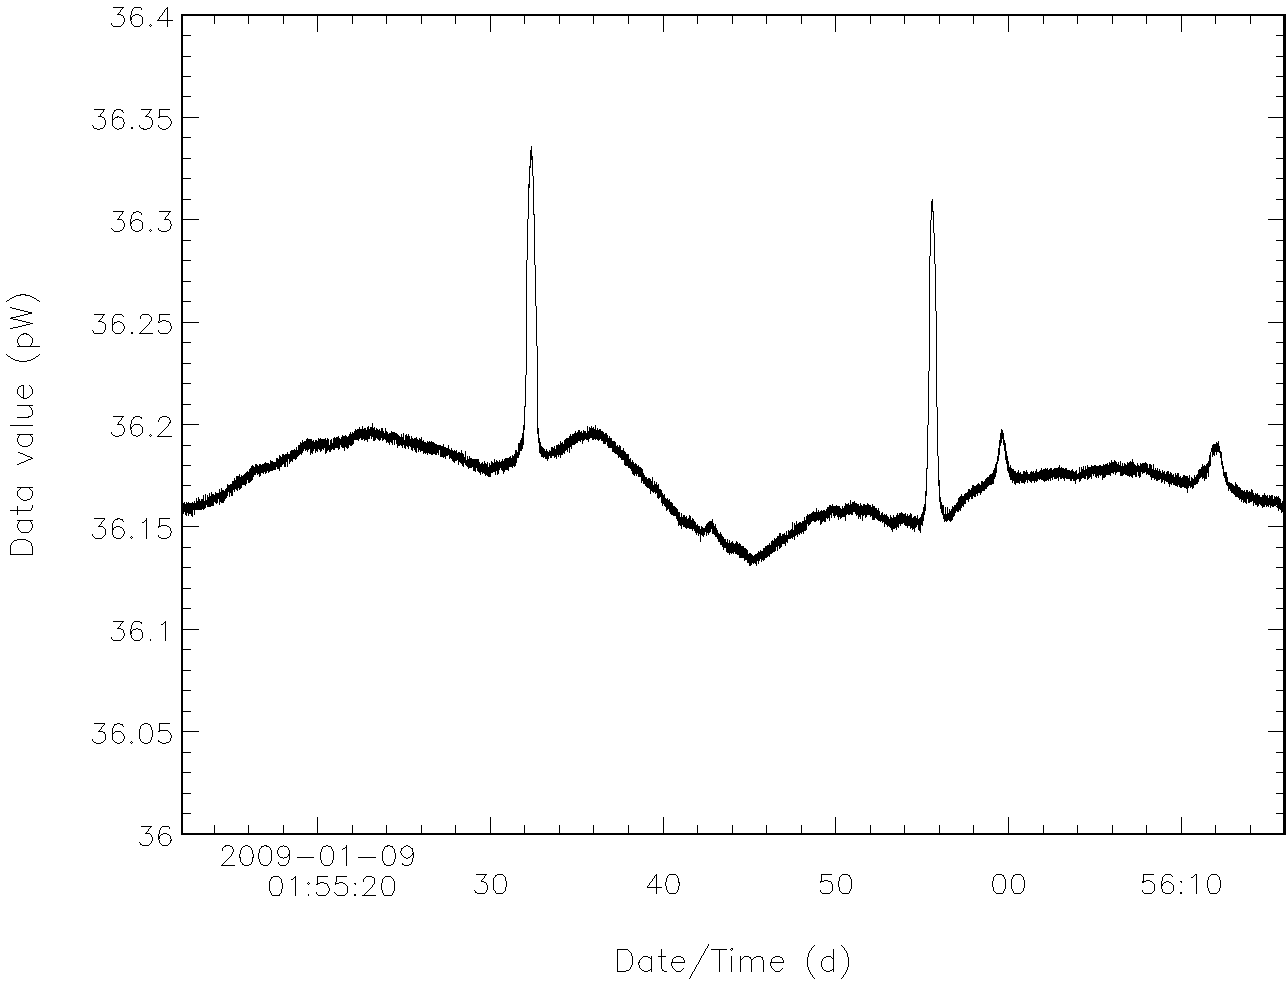
\includegraphics[width=150mm]{sun258_submmsignal}
    \caption{Illustration of the relative magnitudes of atmospheric
      and source signals at submillimetre wavelengths. Data are from
      850 $\mu$m observations of Jupiter with SCUBA-2. The sharp
      features occur when Jupiter is seen by the bolometer. The
      increase in optical power from Jupiter is $\sim$0.5\%. Most
      sources will be many thousands of times fainter.}
    \label{fig:signal}
  \end{center}
\end{figure}

In a single sample the signal collected from an astronomical source is
negligible in comparison with the contribution from the
atmosphere. Many samples are required to collect a statistically
significant signal from the source.

The \SMURF\ routine that removes the sky is called \remsky\ and has
several options for fitting and removing the atmospheric contribution
to the signal. All take advantage of the fact that the sky signal is
correlated between adjacent bolometers.

The atmospheric signal can be fit in the following ways:
\begin{itemize}
\item Calculate the mean value of the signal;
\item Fit a gradient in elevation only;
\item Fit a plane of arbitrary orientation.
\end{itemize}
Furthermore, \remsky\ can make use of the data from all available
sub-arrays simultaneously to make a better estimate of the atmospheric
emission (see the \aparam{GROUP} parameter).

For simple cases, subtracting a mean value may be sufficient, though
it is not recommended for bright sources, as the mean will be biassed
too high by the presence of the source. A more sophisticated solution
may be obtained by fitting a plane to the data. The plane may have
arbitrary orientation (in azimuth and elevation) or may be fixed so
that the slope is in elevation only.

\subsubsection{\xlabel{extinction}Correcting for atmospheric extinction\label{se:extinction}}

This section describes how to correct your data for atmospheric
extinction, the loss of radiation from the source as it travels
through the atmosphere. This step is required for both the full and
simplified workflows.

The observed signal from an astronomical source decreases as the
atmosphere along the line of sight increases. At lower elevations,
there is more atmosphere along the line of sight between the source
and the telescope.

The radiation received by SCUBA-2 is the sum of the radiation from the
astronomical source (represented by $I_{\textrm{src}}$ in Equation
\ref{eq:iobs} below) and the radiation from the atmosphere ($I_{\textrm{atm}}$). However, $I_{\textrm{src}}$ is diminished by the optical depth
of the atmosphere ($\tau$) as follows:
\begin{equation}
I_{\textrm{obs}} = I_{\textrm{atm}} + I_{\textrm{src}} \exp(-\tau).
\label{eq:iobs}
\end{equation}
The optical depth is usually quoted as the value at the zenith
($\tau_{\textrm{zenith}}$), but you need the value of tau at the same
elevation as your observations ($\tau_{\textrm{obs}}$). For a
plane-parallel atmosphere, $\tau_{\textrm{obs}} = A \times \tau_{\textrm{zenith}}$, where airmass ($A$) is a measure of the total atmosphere
along the line of sight.

Airmass is defined as $1 / \cos \theta$, where $\theta$ is the zenith
angle. The zenith angle is the vertical angle measured from the zenith
($\theta = 0^\circ$) towards the horizon ($\theta = 90^\circ$) and is
thus equal to $90-\phi$, where $\phi$ is the elevation. You can now
calculate $\tau_{\textrm{obs}}$ from $\tau_{\textrm{zenith}}$ and $\phi$ as
follows:
\begin{equation}
\tau_{\textrm{obs}} = \tau_{\textrm{zenith}} / \cos(90^\circ - \phi ).
\label{eq:tau}
\end{equation}

Using Equation \ref{eq:tau}, rewrite Equation \ref{eq:iobs} as:
\begin{equation}
I_{\textrm{obs}} = I_{\textrm{atm}} + I_{\textrm{src}} \exp \left(
\frac{-\tau_{\textrm{zenith}}}{\cos(90^\circ-\phi)}\right).
\end{equation}
%The top graph in Figure ??? shows how the observed signal varies with elevation
%and airmass.

The elevation angle of each bolometer can be calculated, and given
$\tau_{\textrm{zenith}}$ \remsky\ calculates the $\tau_{\textrm{obs}}$ at the
elevation angle of each bolometer.

The zenith optical depth can be obtained via three methods:
\begin{enumerate}
\item Skydips: The zenith optical depth is derived from a SKYDIP
  observation, in which the signal at each wavelength is recorded over
  a range of airmasses. \SMURF\ does not yet have the capability to
  process SCUBA-2 skydips.

\item CSO tipping radiometer: The Caltech Submillimeter Observatory
  (CSO) radiometer measures $\tau_{\textrm{zenith}}$ from skydip
  observations at 225 GHz. The CSO radiometer records a new $\tau_{\textrm{zenith}}$ every 10 minutes and values are stored in the FITS
  headers corresponding to the start and end timestamps of the file
  (\texttt{TAU225ST} and \texttt{TAU225EN}). \SMURF\ converts CSO
  $\tau_{\textrm{zenith}}$ to $\tau_{\textrm{zenith}}$ at 450 or 850 $\mu$m,
  relying on an empirical relationship between $\tau_{\textrm{zenith}}$ at
  225 GHz and $\tau_{\textrm{zenith}}$ at 450 or 850 $\mu$m.

\item JCMT Water Vapour Monitor: The JCMT Water Vapour Monitor (WVM)
  provides opacity estimates every 1.2 seconds by measuring the
  spectral shape of the 183 GHz water line along the telescope
  line-of-sight, and then converting this to an effective $\tau_{\textrm{zenith}}$ at 225 GHz. Since the measurement is aligned with the
  submillimetre beam this method circumvents the need to apply the
  plane parallel approximation (which breaks down at the horizon). The
  raw WVM data are stored in the JCMT state structure, though the
  values at times corresponding to the start and end of the file are
  stored in the FITS headers (\texttt{WVMTAUST} and
  \texttt{WVMTAUEN}).
\end{enumerate}
Optical depth measurements derived from the WVM are most useful in
variable atmospheric conditions where the CSO radiometer may not be
giving sufficiently-frequent readings.

The \SMURF\ routine that corrects for atmospheric extinction is called
\extinction. The \extinction\ routine can use $\tau_{\textrm{zenith}}$
determined by all of the above methods, and obtains values
automatically from the FITS headers for the WVM and CSO cases or uses
the raw WVM data if desired.

The user can choose how accurate a correction they wish to apply using
the \aparam{METHOD} parameter. By default, \extinction\ will assess
the magnitude of the correction and if it does not change
significantly across the field of view, then a single value is used
(corresponding to the elevation of the tracking position). If there is
a significant variation, then \extinction\ will apply a correction to
each bolometer using the elevation of that bolometer. It is possible
to enforce either of these options by setting \aparam{METHOD} to
\texttt{QUICK} or \texttt{FULL} respectively.

Note that sky subtraction must take place before the extinction
correction is applied. \extinction\ checks the history to see if
\remsky\ has been run and exits with an error if not. However, if an
alternative method of sky subtraction has been used (such as using
\KAPPA\ \csub\ to subtract a mean or median value) then the
\aparam{HASSKYREM} may be set to \texttt{TRUE} to override the history
check by \extinction.

\subsubsection{\xlabel{dsimages}Calculating images from time-series
  data\label{se:dsimages}}

This step is not required for the simplified workflow.

\SMURF\ provides separate routines for calculating images from STARE
and DREAM data. STARE images are calculated with \starecalc; DREAM
images are calculated with \dreamsolve.

In \starecalc\ the user may specify how many samples to average to
create images (the default is to calculate averages once a second).

\dreamsolve\ requires the DREAM weights file specified in the FITS
header keyword \texttt{DRMWGHTS} to reside in the current
directory. Data from each sub-array require a corresponding weights
file. See section \ref{se:dream} below for details on calculating
alternative weights files.

\subsubsection{\xlabel{mosaic}Combining the images\label{se:mosaic}}

\SMURF\ does not have any image mosaicking tasks itself. This step is
handled by routines in \KAPPA\ and \CCDPACK. Suitable tasks are
\wcsmosaic\ in \KAPPA\ and a combination of \KAPPA\ \wcsalign\ (to
align all the images to a common coordinate frame) followed by
\CCDPACK\ \makemos.

See the SCUBA-2 cookbook (\SMURFcook) for more detailed information
about mosaicking SCUBA-2 images.

\subsubsection{\xlabel{dream}Using alternative DREAM solutions\label{se:dream}}

This step is not usually necessary for either workflow but is included
for completeness.

The DREAM observing mode moves the secondary mirror in a pattern which
causes adjacent bolometers to observe the same region of the sky
multiple times \cite{scuba2,dream}. The data are then described by a
series of simultaneous equations which are solved via a matrix
inversion (using singular value decomposition). Since the pattern
traced out by the secondary mirror is known, the inverse of the matrix
can be pre-calculated (a time-consuming task) for a given output grid
and applied to data at the time of observation (quick).

It is \emph{strongly} recommended that users become familiar with the
details of DREAM \cite{dream} before using weights other than the
default for science data processing.

The user may wish to experiment with different regridding schemes or
there may be other reasons, not known at the time of observation,
which require the inverse matrix to be re-calculated. The task for
doing this is called \dreamweights, and this allows the user to
specify different output grid parameters. The calculation of the
inverse is moderately time-consuming (compared with calculating the
images) and takes of order 5--10 minutes on current hardware. The
output file from \dreamweights\ is the weights file required by
\dreamsolve. \KAPPA\ \fitsedit\ may be used to specify weights files
which differ in name from the default. Note that this process must be
repeated for each sub-array for which data exist and that data which
are to be combined should all use the same grid.

\subsection{Moving sources}

Mosaicking of DREAM and STARE images of moving sources will require the WCS
attributes \verb+AlignOffset+ and \verb+SkyRefIs+ to be changed to 1
and `origin' respectively. Use the \KAPPA\ task \wcsattrib\ to
modify these attributes.


\section{\xlabel{rebin}Rebinning map-maker\label{se:rebin}}

The processing of SCAN data with the rebin method proceeds in a
multi-step approach that follows the method listed above for DREAM and
STARE data using \makemap. A one-pass rebinning algorithm is applied
to the data, which regrids the signal from each bolometer on to a map
in the desired co-ordinate system.

As outlined in \ref{se:dsworkflow}, the procedure for processing
SCUBA-2 data follows these steps:
\begin{enumerate}
\item Apply the flatfield correction (see Section \ref{se:flatfield});
\item Clean the data set using \clean. This can remove spikes, DC
  steps and low- and high-frequency components in the data.
\item Remove the contribution of atmosphere to the signal (see Section
  \ref{se:skysub});
\item Correct for atmospheric extinction (see Section
  \ref{se:extinction});
\item Make a map using the rebin method.
\end{enumerate}

The rebinning algorithm shares the observed signal from a single
bolometer between neighbouring output map pixels, as determined by the
pixel-spreading function. The value of each pixel in the map is the
sum of the signal from every bolometer that observed at that position.

There are many options for the pixel spreading scheme (see the \wcsmosaic\
documentation for a summary). The fastest option is to use the nearest-neighbour
pixel spreading scheme (`Nearest'), which assigns the whole signal
from one bolometer to the nearest map pixel. This option does not
always produce smooth maps (if the map is poorly sampled, for example,
but it produces a robust estimate of the noise. In the limit of a
large number of `hits' per pixel, and with a pixel size sufficiently
small compared to the beamsize, this method is optimal.

For smoother maps (with poor sampling, for example), the `Linear'
scheme can be used to share the input signal equally among the four
nearest map pixels. There are more complicated options available,
e.g., Sinc-type functions, or Gaussian distributions. These methods
produce aesthetically pleasing maps, at the risk of introducing
correlations into the noise and additional smoothing to the map.

Figure \ref{fig:rebinmap} shows an example map created from simulated
observations of an extended source with bright features. It was
created using the rebin method and the nearest-neighbour pixel
spreading scheme.

Note the dark regions around the bright sources. They are negative
bowls introduced by the sky subtraction method (Section
\ref{se:skysub}). The random dots are cosmic ray spikes which are not
removed by this particular workflow.

\begin{figure}[htb]
  \begin{center}
    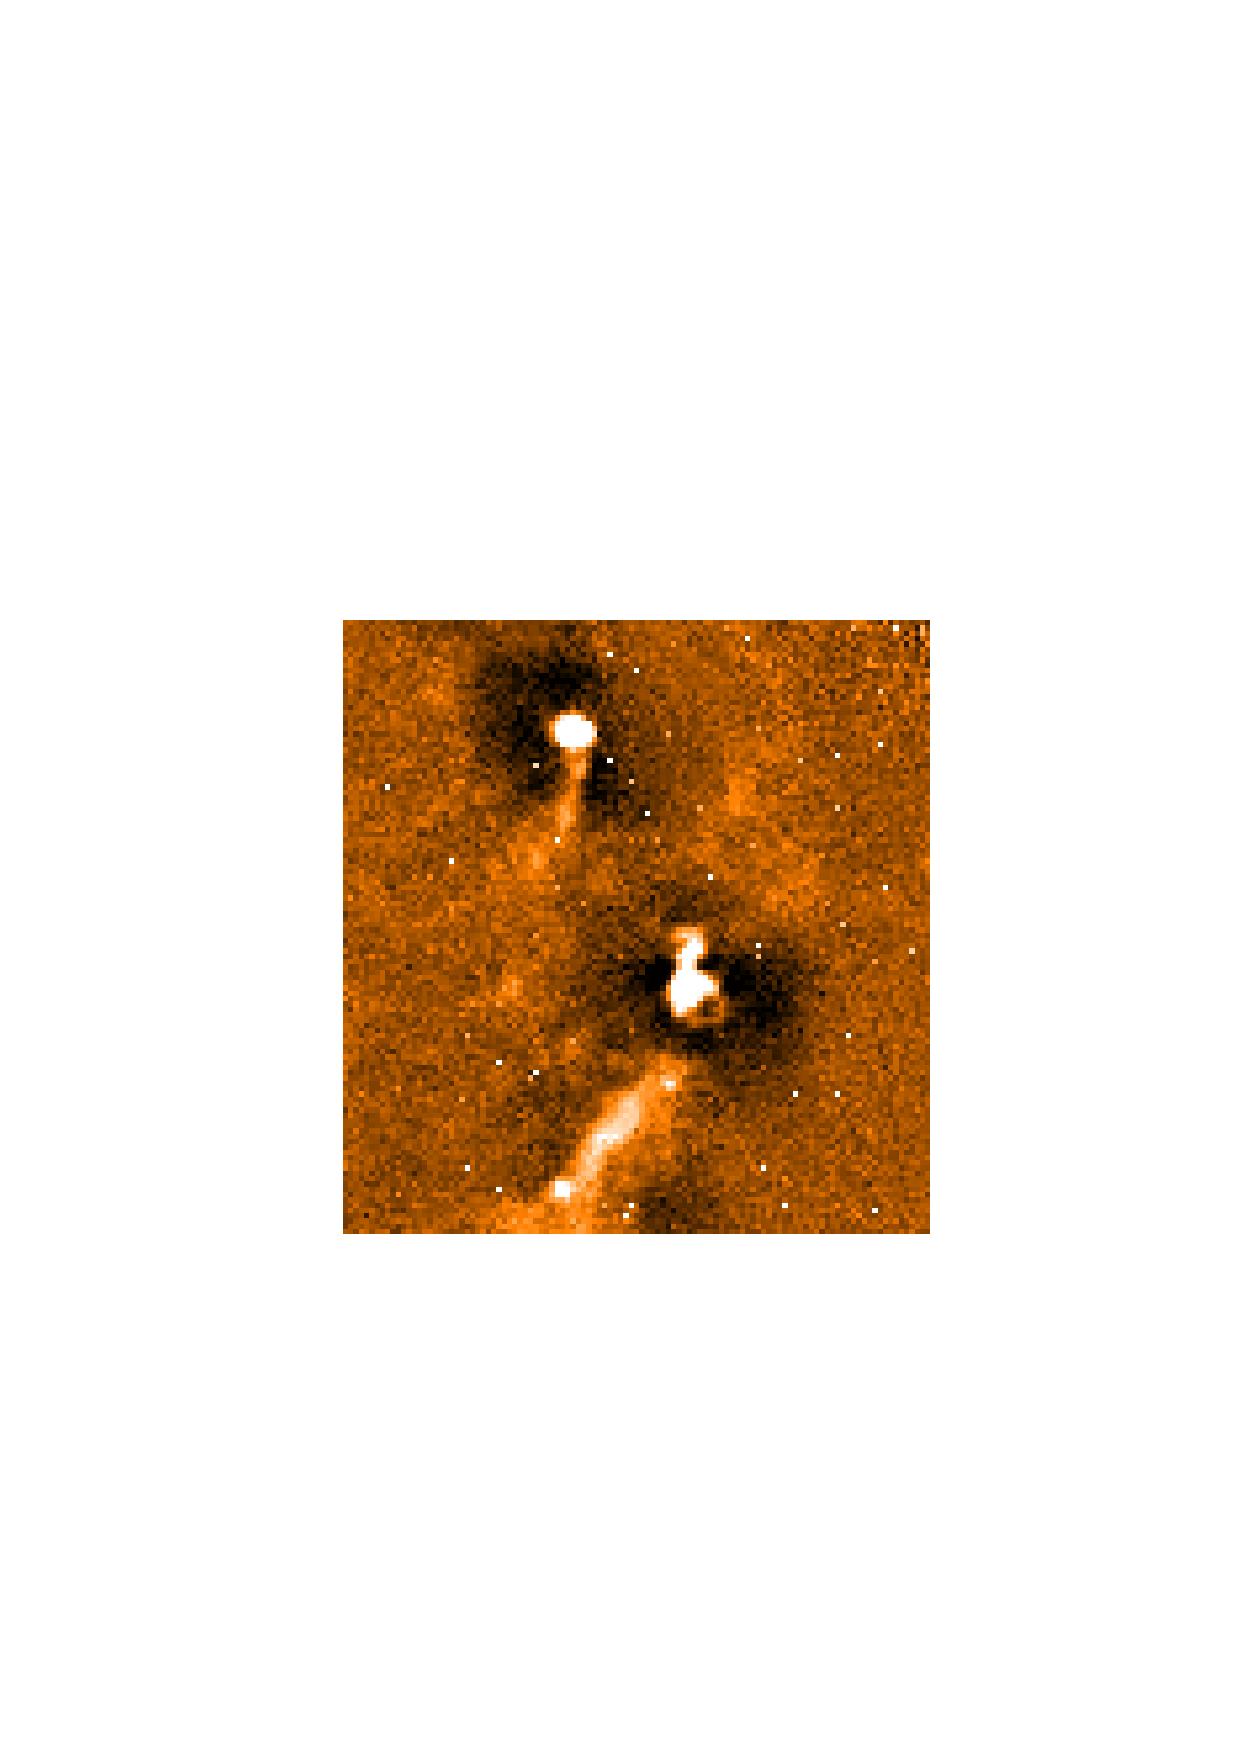
\includegraphics[width=0.7\linewidth]{sun258_rebinmap}
    \caption{Image reconstructed from simulated data using the
      \aparam{REBIN} method. Note the deep wells around bright
      sources and the numerous spikes caused by (simulated) cosmic
      rays.}
    \label{fig:rebinmap}
  \end{center}
\end{figure}


\section{\xlabel{simulator}SCUBA-2 Simulator\label{se:sc2sim}}

\SMURF\ has the capability to produce simulated data from SCUBA-2 with
the \sctwosim\ task. The simulator samples an input astronomical image
in the presence of a model atmosphere and other sources of noise.
Output files are written in the same format as real data from SCUBA-2
with complete flatfield, WVM, WCS and JCMT state structure
information. These files can be processed with other \SMURF\
tasks. Model atmospheres may be generated with the \skynoise\ task.

The simulator supports the primary observing modes: DREAM, STARE and
SCAN along with FLATFIELD, POINTING and FOCUS
observations. Rudimentary support exists for the SCUBA-2 polarimeter
though this is untested. Instrument apertures may be set (offsets
which adjust the tracking position to a specific sub-array), and
microsteps (small offsets from the tracking position) are fully
supported. Simulating the motion of the major Solar System bodies
(Venus, the Moon, Mars, Jupiter, Saturn, Uranus and Neptune) is
supported.

For SCAN observations, the simulator has two modes controlled by the
\texttt{SIMTYPE} parameter. A \texttt{FULL} simulation generates
simulated complete astronomical data including the effect of the
atmosphere. A \texttt{WEIGHTS} simulation generates data which may be
used to assess areal coverage and `hit' density (i.e.\ the number of
times a point on the sky is observed) for different mapping strategies
or the impact of non-working bolometers. Several different scanning
models are supported: boustrophedon (conventional back-and-forth
raster scan), two variations of `pong' (or box-scan) with either
sharp or gentle turnarounds and a lissajous pattern. [REF TO ANA SCAN DOC]

\subsection{\xlabel{simuse}Simulator workflow\label{se:simuse}}

The simulator requires some preparatory work before data can be
simulated. The basic procedure is outlined below:
\begin{itemize}
\item Obtain an astronomical sky image;
\item Calculate a model atmosphere;
\item Calculate a flatfield solution;
\item Decide on simulation parameters;
\item Run simulation.
\end{itemize}
It is not necessary to recalculate a model atmosphere or flatfield
solution for every simulation, even for different input sky images.

Example files are installed as part of \SMURF\ and may be found in the
\texttt{\$STARLINK\_DIR/share/smurf} directory. An explanation may be
found in the \texttt{README} file in that directory.

\subsubsection{Astronomical image}

The astronomical image may be any suitable image, provided it has WCS
information. It should be as large as the size of the map to be
made. The WCS is used unless the source is a moving object (listed
above). The image must be an NDF. It is recommended that the image
pixel scale be set to be much less than the likely output map pixel
spacing (typically 3 arcsec at 850 $\mu$m, 1 arcsec at 450 $\mu$m) to
avoid imaging and sampling artefacts.

\subsubsection{Model atmosphere}

The model atmosphere is calculated with the \skynoise\ task. The
atmosphere is modelled as a Kolmogorov turbulent thin-screen
\cite{sc2ana002} with a characteristic turnover frequency and scaling
law. Different models may be generated for the same parameters using a
random number seed (specified or calculated internally using the
system clock). The parameters may be modified though the user should
be familiar with the details of this model of the atmosphere before
exploring the parameter space too widely.

The model atmosphere calculated is generic and may be used for
simulations at both 850 $\mu$m and 450 $\mu$m. The model is scaled
at the time of simulation according to the particular wavelength.

\subsubsection{Flatfield simulation}

Before a data simulation can take place, the flatfield solution for
each sub-array must be calculated. This is achieved by specifying a
special observing mode called \texttt{heatrun} and running a
simulation.

The flatfield solution is written to a file using a naming scheme
which follows that for raw data. The convention is
\verb+s[4|8][a-d]heatYYYYMMDD_NNNNN.sdf+ where \verb+s[4|8][a-d]+ is
the sub-array name (e.g.\ \verb+s8a+), \verb+heat+ indicates a
flatfield observation, \verb+YYYYMMDD+ is the date of observation and
\verb+NNNNN+ is a zero-padded, 5-digit observation number.

The simulator relies on this naming scheme for reading the flatfield
information, and the files must be present in the current directory.

\subsubsection{Running the simulator}

The simulator has a large number of parameters which may be freely
adjusted. The list of parameters is divided between two groups:
simulation parameters (usually telescope- and instrument-specific); and
observation parameters (properties of the observation in
question). These are specified using the \texttt{SIMPAR} and
\texttt{OBSPAR} ADAM parameters to \sctwosim. For convenience, the
parameters are stored in plain text files and are passed in using the
\verb+^+ scheme mentioned above in Section \ref{se:files}. Example
input files for all major observing modes may be found in the
\texttt{\$STARLINK\_DIR/share/smurf} directory.

The main observation parameters (\texttt{OBSPAR}) of interest are the
RA/Dec of the source, wavelength, observing mode (\texttt{obsmode}),
observation date and duration of observation (which in the case of
SCAN observations, is determined by the size of the area to
map). Planets may be specified by name. The RA/Dec must match that in
the astronomical image. If the source is not above the horizon, the
simulator will exit with an error message. The date must be specified
as a UT modified Julian day number. As a point of reference,
20090701T00:00:00 corresponds to MJD 55013.

The main simulation parameters (\texttt{SIMPAR}) are the sub-arrays to
simulate data for, the names of the atmosphere model and astronomical
source files and the zenith opacity (at 225 GHz). The zenith opacty is
converted to a value at the appropriate wavelength using the empirical
relations derived for SCUBA by Archibald et al. (2002). Similar
relations for SCUBA-2 will be derived.

Data for all sub-arrays (at the specified wavelength) may be generated
in a single run. The size of the output files is governed by the
\texttt{MAXWRITE} parameter for \sctwosim\ which specifies the number
of samples to write per file. Multiple observations may be simulated
by setting the \texttt{OVERWRITE} parameter to \texttt{FALSE} (the
default behaviour is to overwrite existing files).

A word of caution. Since the data output from the simulator mimics the
real instrument, it is possible to generate many GB of data which may
take many minutes to hours of CPU time. The \sctwosim\ parameter
\texttt{SIMSTATS} tells the simulator to estimate the properties of
the simulation including the duration of the simulation, quantity of
data, memory requirements and CPU time. The results are printed to the
screen, allowing the user to modify the simulation parameters if
necessary.

\subsubsection{\xlabel{dreamsim}A note on DREAM simulations\label{se:dreamsim}}

For STARE simulations, the images are calculated at 1-second intervals
at the time the simulator is run and written to the output files. For
DREAM the images must be reconstructed after the simulation has
run. This means that the DREAM weights file must be calculated using
\dreamweights\ as desribed in Section \ref{se:dream}. Likewise, the
images are calculated using \dreamsolve.

\subsection{\xlabel{simdr}Processing simulated data\label{se:simdr}}

The processing of simulated data proceeds exactly as for real SCUBA-2
data and depends on the observing mode. See the respective workflows
in Sections \ref{se:dsworkflow} and \ref{se:dimm} above. Note
that dark frames are not produced by the simulator and do not need to
be included in any processing (there is no drift in the model
bolometer response).

FOCUS observations are designed to be processed by the \ORACDR\
pipeline rather than \SMURF, as their analysis involves multiple
steps. POINTING observations are equivalent to short science
observations and should be processed in the same way.


\end{document}

